%Tema para beamer "CCM3" versión 1
%Desarrollo por Erick David Luna Núñez y 
%Fernanda Barajas Hernandez

\documentclass{beamer}

\usepackage[utf8]{inputenc}
\usepackage{heuristica}
\usepackage[T1]{fontenc}
\usepackage[heuristica,vvarbb,bigdelims]{newtxmath}
\renewcommand*\oldstylenums[1]{\textosf{#1}}
\usepackage[sfdefault,scaled=.85]{FiraSans}
\usepackage{graphicx}
\usepackage[spanish]{babel} 
\usepackage[pages=some]{background}
\pagenumbering{arabic}

%~~~~~~~~~~~~~~~~~~~~~~~~~~~~~~~~~~~~~~~~~~~~~~~~~~~~~~~~~~~~~~~~~~~~~~~~~~~~~~
% Include Figure
\usepackage{graphicx}
%\usepackage{figure}
\usepackage{subcaption}
\usepackage{wrapfig}
%~~~~~~~~~~~~~~~~~~~~~~~~~~~~~~~~~~~~~~~~~~~~~~~~~~~~~~~~~~~~~~~~~~~~~~~~~~~~~~


%%Se define el "environment" teorema
\newtheorem{teorema}{Teorema}
% Proof
\renewcommand*{\proofname}{\textbf{Demostraci\'on:}}
% Lemma
\newtheorem{lema}{Lema}

% Conjetura
\newtheorem{conjetura}{Conjetura}

%Definir el autor con el estilo definido (el textbf y el uso del color son herramientas del diseño, no necesario borrar)
\title{\Large {Geometría Computacional}\\ {\color{mostazaccm} \textbf{Problemas de iluminación y visualización.}}}

%Nombre del autor
\author{Adrián Aguilera Moreno.} 

%Fecha o evento en que se presentará la plática
\date{\\\textbf{Profesores:}
  \\ {Adriana Ramírez Vigueras}
  \\ {Marco Antonio Velasco Flores}
  \\ {Fhernanda Montserrat Romo Olea}} 

%correo del expositor o incluir posibles colaboradores
\institute{aguilera@ciencias.unam.mx} 


%%Tema de beamer "CCM-3"
\usetheme{ccm3}

\begin{document}
%Define el fondo de la primer diapositiva
{\setbeamertemplate{background}{

\includegraphics[width=\the\paperwidth,height=\the\paperheight]{images/P3.png}}
%lo anterior es para definir el fondo de la primer diapositiva

\begin{frame}
  \titlepage %Necesario para generar la portada
\end{frame}

} %aquí termina el cambio de fondo

\begin{frame}
\tableofcontents %Imprime la tabla de contenido
\end{frame}

\section{Introducción} %%Título de la sección (Opcional)
\subsection{Iluminación y Visualización.}
% Introducción
\begin{frame}
  \frametitle{Introducción}
  \framesubtitle{Problemas de iluminación.} %%Subtítulo de la diapositiva (opcional)
  Un problema de iluminación consta de iluminar áreas específicas con fuentes. Las fuentes de luz
  utilizadas para iluminar nuestros objetos pueden ser de varios tipos, lámparas que emiten luz
  alrededor de ellas, reflectores o fuentes de luz que solo iluminan dentro de una zona angular, etc.

  %\centering \includegraphics[width=0.35 \paperwidth]{images/Iluminación.png}
  \begin{figure}
    \centering
    \includegraphics[width=0.35 \paperwidth]{./images/Iluminación.png}
    \caption*{Iluminación.}
  \end{figure}
  
  %\begin{itemize}
  %  \item[\checkmark] Un elemento en la lista %%[\checkmark] muestra una palomita al inicio de la línea
  %  \item Segundo elemento
  %  \item Otro elemento
  %  \item Y finalmente, otro más
  %\end{itemize}
\end{frame}

\begin{frame}
  \frametitle{Introducción}
  \framesubtitle{Problemas de visualización.} %%Subtítulo de la diapositiva (opcional)
  Intimamente ligado a los problemas de iluminación está el estudio de gráficas
  de visibilidad. Dado un polıígono $P$ en el plano, la gráfica de visibilidad
  interna de $P$ es la gráfica cuyos vértices son los vértices de $P$, en la cual dos
  vértices son adyacentes, si el segmento de línea que los une está totalmente
  contenido en $P$ (análoga la definición externa).

  %\centering \includegraphics[width=0.35 \paperwidth]{images/Iluminación.png}
  \begin{figure}
    \centering
    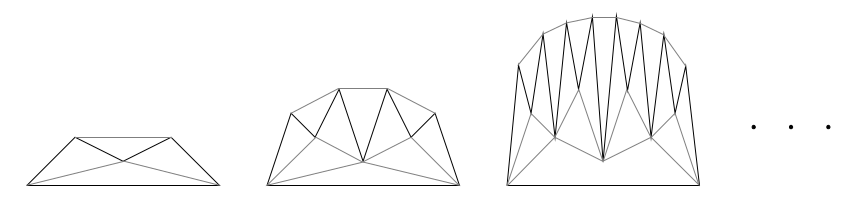
\includegraphics[width=0.55 \paperwidth]{./images/GraphVisibility.png}
    \caption*{Gráficas de visibilidad en una familia de polígonos.}
  \end{figure}
  
  %\begin{itemize}
  %  \item[\checkmark] Un elemento en la lista %%[\checkmark] muestra una palomita al inicio de la línea
  %  \item Segundo elemento
  %  \item Otro elemento
  %  \item Y finalmente, otro más
  %\end{itemize}
\end{frame}



\section{Iluminando Polígonos Ortogonales.}
\subsection{Antecedentes.}
% Introducción
\begin{frame}{Polígonos Ortogonales.} %%Otra forma (más corta) de poner el título a la diapositiva
  Un polígono simple en el plano se llama ortogonal si sus aristas son paralelas a los
  ejes coordenados.
  
  \begin{figure}
    \centering
    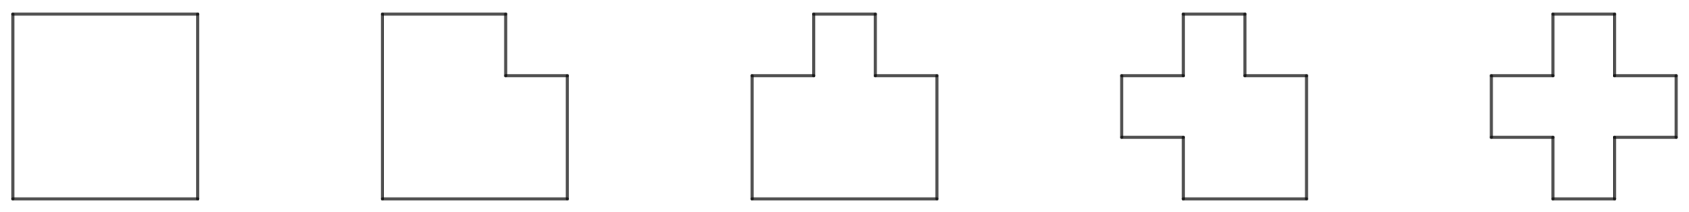
\includegraphics[width=.8 \paperwidth]{./images/EOrtogonales.png}
    \caption*{Ejemplos de polígonos ortogonales.}
  \end{figure}
\end{frame}

% Antecedente 1:
\begin{frame}{Antecedente I.} %%Otra forma (más corta) de poner el título a la diapositiva
  \framesubtitle{¿Cuántos vértices concavos hay en un polígono ortogonal?} %%Subtítulo de la diapositiva (opcional)
  Sabemos que los ángulos en un polígono ortogonal son $\frac{\pi}{2}$ o $\frac{3\pi}{2}$. Los vértices
  concavos son siempre de $\frac{3\pi}{2}$. \newline
  
  \textbf{Lema.} Todo polígono ortogonal con $n$ vértices tine
  $\frac{n - 4}{2}$
  vértices concavos.
  
  \begin{proof}
    Procedamos por inducción sobre el número de vértices. Es fácil ver que sólo podemos agregar $2m$ vértices
    a la vez, con $m \in \mathbb{Z}$. Supongamos que para $k$ vértices se cumple el lema. ¿Qué pasa con $k + 2$
    vértices?
    \[\frac{k - 4}{2} + 1 = \frac{k - 4 + 2}{2} = \frac{(k + 2) - 4}{2}.\]
  \end{proof}
\end{frame}

% Antecedente 2:
\begin{frame}{Antecedente II.} %%Otra forma (más corta) de poner el título a la diapositiva
  \framesubtitle{Clasificando vértices y aristas.} %%Subtítulo de la diapositiva (opcional)
  \begin{figure}
    \centering
    \begin{subfigure}[b]{0.4\paperwidth}
      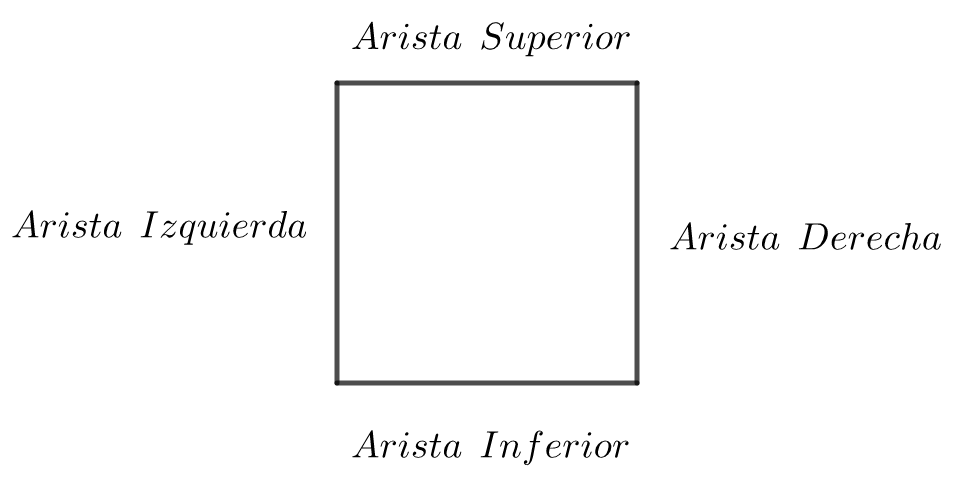
\includegraphics[width=0.4\paperwidth]{./images/CAristas.png}
      \caption*{Clasificación de aristas.}
    \end{subfigure}
        \begin{subfigure}[b]{0.4\paperwidth}
      \includegraphics[width=0.4\paperwidth]{./images/CVértices.png}
      \caption*{Clasificación de Vértices.}
    \end{subfigure}
  \end{figure}
\end{frame}

% Antecedente 3:
\begin{frame}{Antecedente III.} %%Otra forma (más corta) de poner el título a la diapositiva
  \framesubtitle{Clasificando vértices y aristas.} %%Subtítulo de la diapositiva (opcional)
  \begin{figure}
    \centering
    \includegraphics[width=0.8\paperwidth]{./images/Clasificación completa.png}
    \caption*{Clasificando aristas y vértices.}
  \end{figure}
\end{frame}

% Antecedente 4:
\begin{frame}{Antecedente IV.} %%Otra forma (más corta) de poner el título a la diapositiva
  \framesubtitle{Corte impar.} %%Subtítulo de la diapositiva (opcional)
  \textbf{Def.} Dado un polígono ortogonal $P$, definimos un \textit{corte horizontal} o \textit{vértical}
  de $P$, como la extensión de una arista horizontal o vértical de $P$ a partir de un vértice concávo hacia
  el interior de $P$ hasta un punto de intersección con la frontera de $P$.
  \begin{figure}
    \centering
    \begin{subfigure}[b]{0.2\paperwidth}
      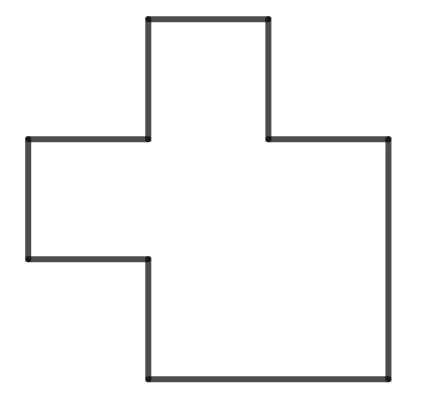
\includegraphics[width=0.1\paperwidth]{./images/Fig.png}
      \caption*{Polígono.}
    \end{subfigure}
    \begin{subfigure}[b]{0.2\paperwidth}
      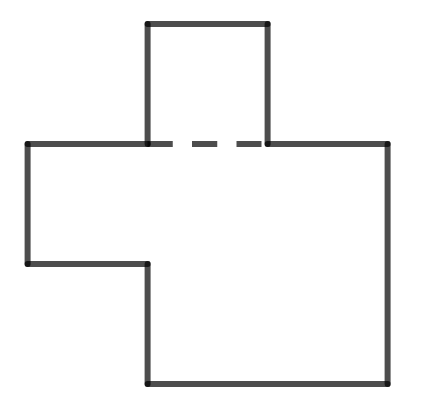
\includegraphics[width=0.1\paperwidth]{./images/FigCH.png}
      \caption*{Corte horizontal.}
    \end{subfigure}
    \begin{subfigure}[b]{0.2\paperwidth}
      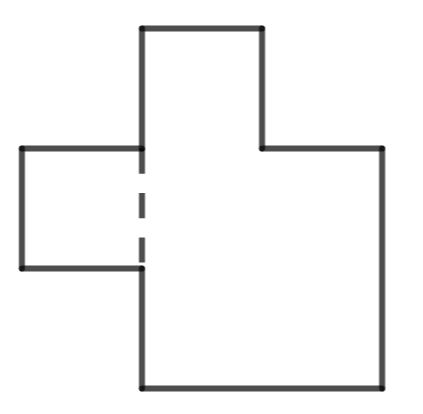
\includegraphics[width=0.1\paperwidth]{./images/FigCV.png}
      \caption*{Corte vértical.}
    \end{subfigure}
  \end{figure}
  \textbf{Def.} Un corte impar es un corte horizontal o vértical, tal que uno de los subpolígonos
  que forma es de tamaño $4k + 2$. Con $k \in \mathbb{Z}$.
\end{frame}

\subsection{Lámparas suficientes para iluminar polígonos ortogonales.}
% Problema:
\begin{frame}{El problema.} %%Otra forma (más corta) de poner el título a la diapositiva
  \framesubtitle{¿Cuántas lámparas son necesarias para iluminar?} %%Subtítulo de la diapositiva (opcional)
  \begin{teorema}
    $\lfloor \frac{n}{4} \rfloor$ lámparas son siempre son siempre suficientes y a veces necesarias
    para iluminar cualquier polígono ortogonal con $n$ vértices.
  \end{teorema}
\end{frame}

% Demostración:
\begin{frame}{El problema.} %%Otra forma (más corta) de poner el título a la diapositiva
  \framesubtitle{¿Cuántas lámparas son necesarias para iluminar?} %%Subtítulo de la diapositiva (opcional)
  \textbf{Demostración:}
    Sea $P$ de al menos $8$ vértices. Sean $S_1$ y $S_2$ conjuntos tales que contengan los vértices superiores derechos; inferiores izquierdos
    y los superiores izquierdos; inferiores derechos, respectivamente. $S_1$ o $S_2$ contiene a lo más $\lfloor \frac{n}{4} \rfloor$ vértices
    concavos. Supongamos que es $S_1$ quién contiene a lo más $\lfloor \frac{n}{4} \rfloor$ vértices concavos.
    Si esos vértices iluminan a $P$, entonces terminamos.\newline
    
    Supongamos que los vértices concavos de $S_1$ no iluminan $P$. Entonces, mostremos que existe un corte vértical u horizontal impar.
    Sean, $p \in P$ tal que no es iluminado por algún $s \in S_1$; c un segmento horizontal (vértical) más largo que contiene a $p$;
    $e, f$ aristas de $P$ que contienen los extremos de $c$. $R$ es el rectángulo más grande contenido en $P$ con lados paralelos a
    los ejes coordenados que contenga a $c$.\newline
\end{frame}

\begin{frame}{El problema.} %%Otra forma (más corta) de poner el título a la diapositiva
  \framesubtitle{¿Cuántas lámparas son necesarias para iluminar?} %%Subtítulo de la diapositiva (opcional)
  \textbf{Obs.} Sean $q, q'$ los vértices \textit{superior derecho} e \textit{inferior izquierdo} respectivamente.
  Si $q, q' \in V_P \rightarrow P = R$.

  \begin{figure}
    \centering
    \begin{subfigure}[b]{0.59\paperwidth}
      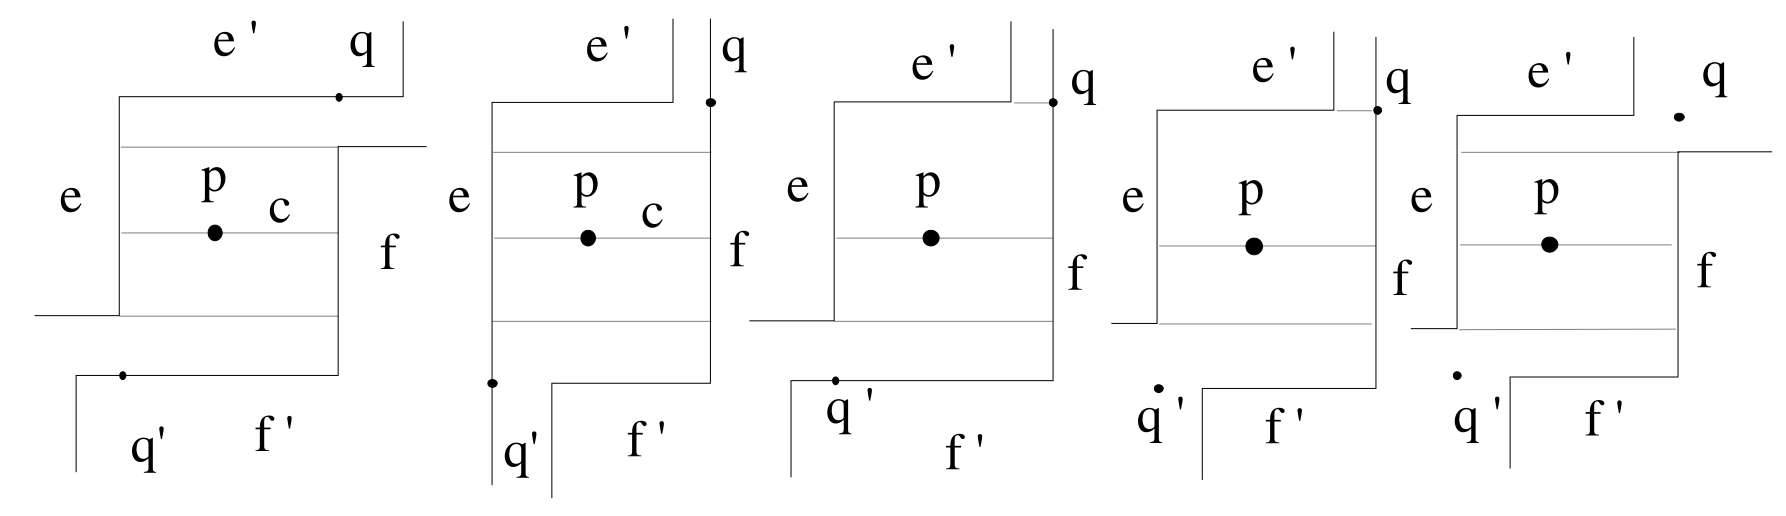
\includegraphics[width=.6 \paperwidth]{./images/CasosOrtogonales.png}
    \end{subfigure}
    \begin{subfigure}[b]{0.1\paperwidth}
      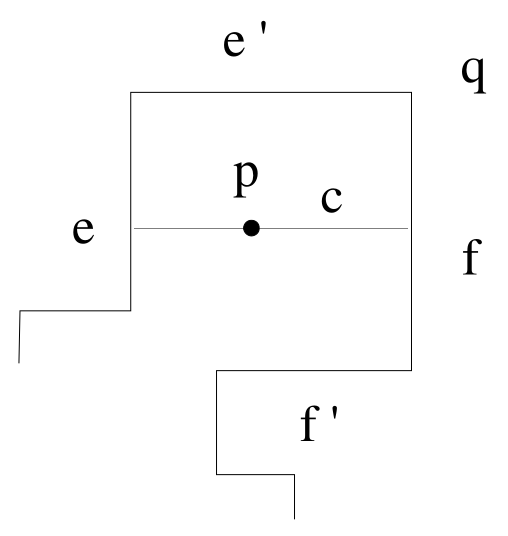
\includegraphics[width=.16 \paperwidth]{./images/CasoOrtogonal.png}
    \end{subfigure}
    \caption*{Casos generados por $q$ y $q'$.}
  \end{figure}
\end{frame}

\begin{frame}{El problema.} %%Otra forma (más corta) de poner el título a la diapositiva
  \framesubtitle{¿Cuántas lámparas son necesarias para iluminar?} %%Subtítulo de la diapositiva (opcional)
  Analicemos $2$ posibles casos:
  \begin{itemize}
  \item $q$ y $q'$ no son vértices de $P$.
  \item Exactamente uno de ellos, digamos que $q$, es vértice de $P$.
  \end{itemize}
  \begin{figure}
    \centering
    \begin{subfigure}[b]{0.59\paperwidth}
      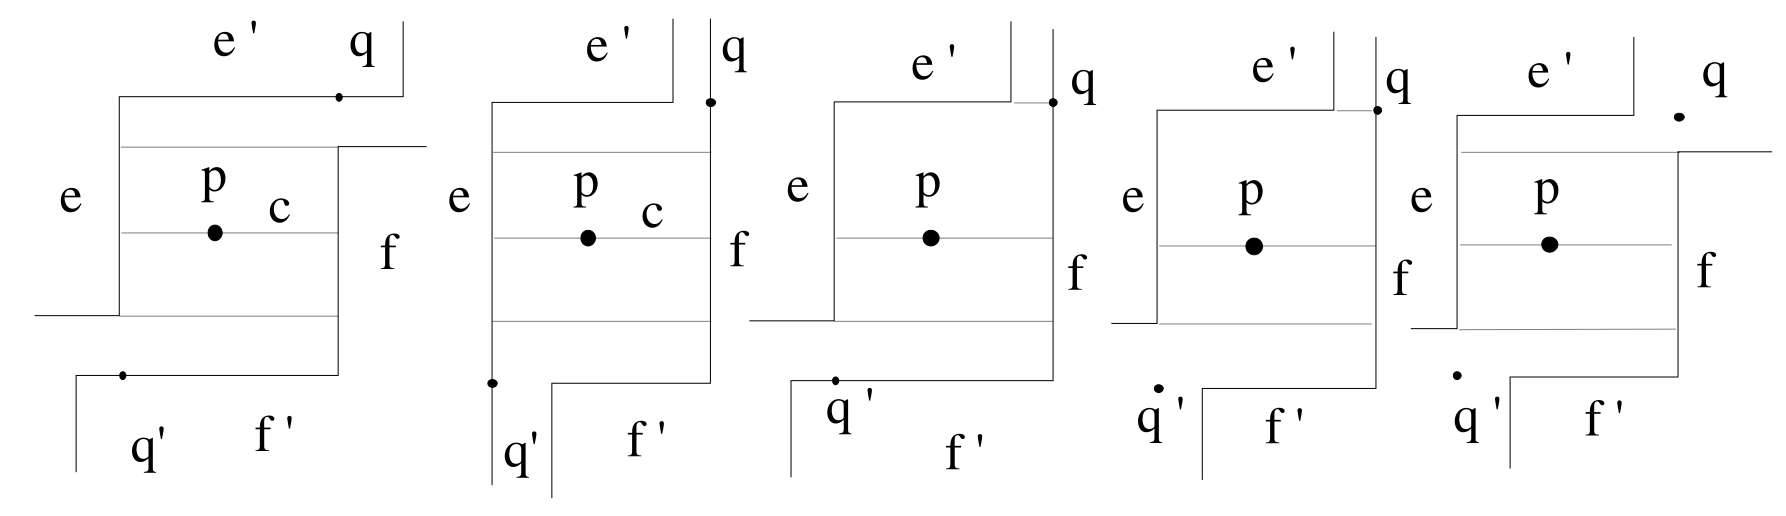
\includegraphics[width=.6 \paperwidth]{./images/CasosOrtogonales.png}
    \end{subfigure}
    \begin{subfigure}[b]{0.1\paperwidth}
      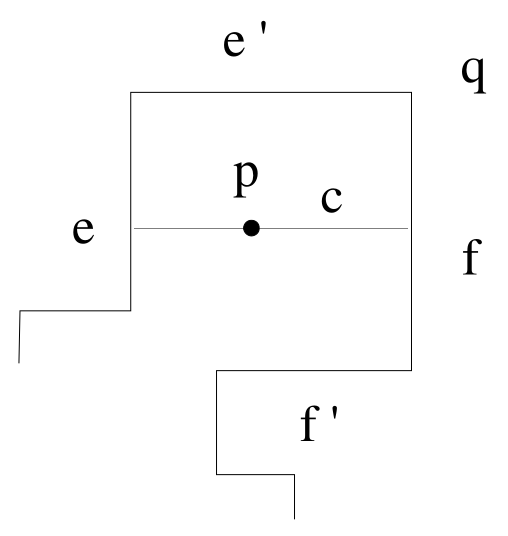
\includegraphics[width=.16 \paperwidth]{./images/CasoOrtogonal.png}
    \end{subfigure}
    \caption*{Casos generados por $q$ y $q'$.}
  \end{figure}
\end{frame}

\begin{frame}{El problema.} %%Otra forma (más corta) de poner el título a la diapositiva
  \framesubtitle{¿Cuántas lámparas son necesarias para iluminar?} %%Subtítulo de la diapositiva (opcional)
  Para el caso (1) es fácil ver que podemos generar dos cortes vérticales (horizontales) en $P$ que generen $R$
  o un rectángulo contenido en el y que contiene a $c$. Es sencillo observar que al menos un corte es impar.
  \begin{figure}
    \centering
    \begin{subfigure}[b]{0.25\paperwidth}
      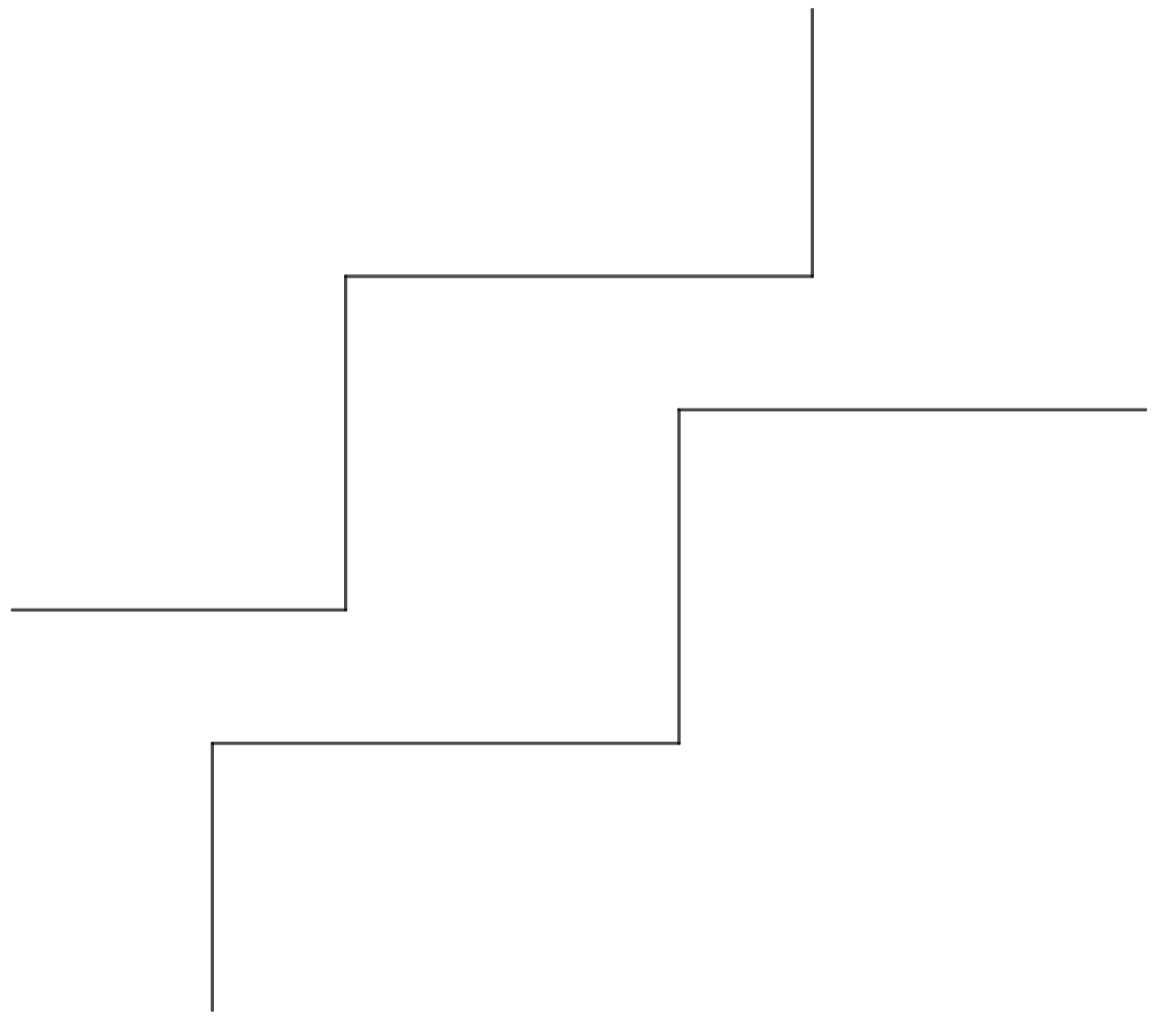
\includegraphics[width=.3 \paperwidth]{./images/Ejemplar.png}
    \end{subfigure}
    \begin{subfigure}[b]{0.25\paperwidth}
      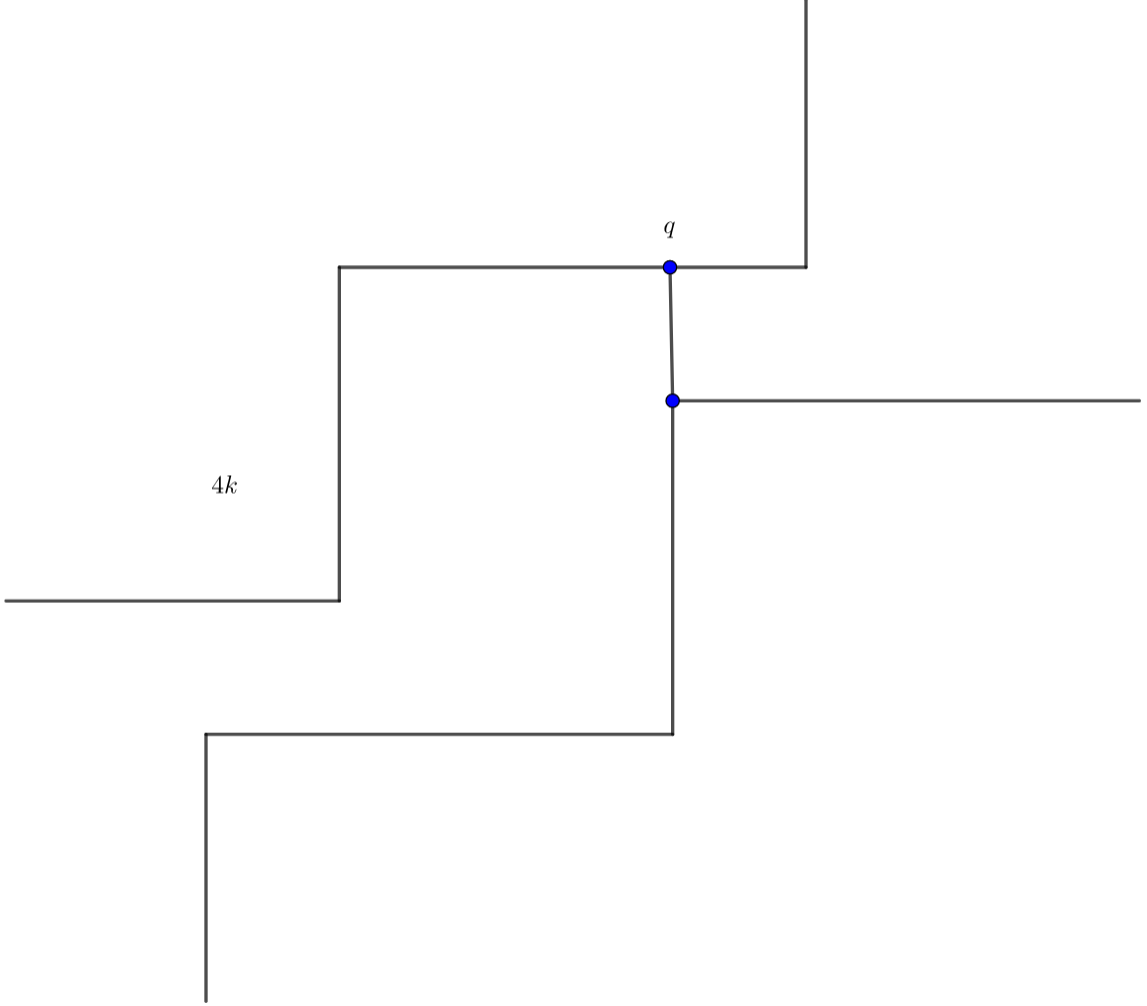
\includegraphics[width=.3 \paperwidth]{./images/EjemplarC1(4k).png}
    \end{subfigure}
    \begin{subfigure}[b]{0.25\paperwidth}
      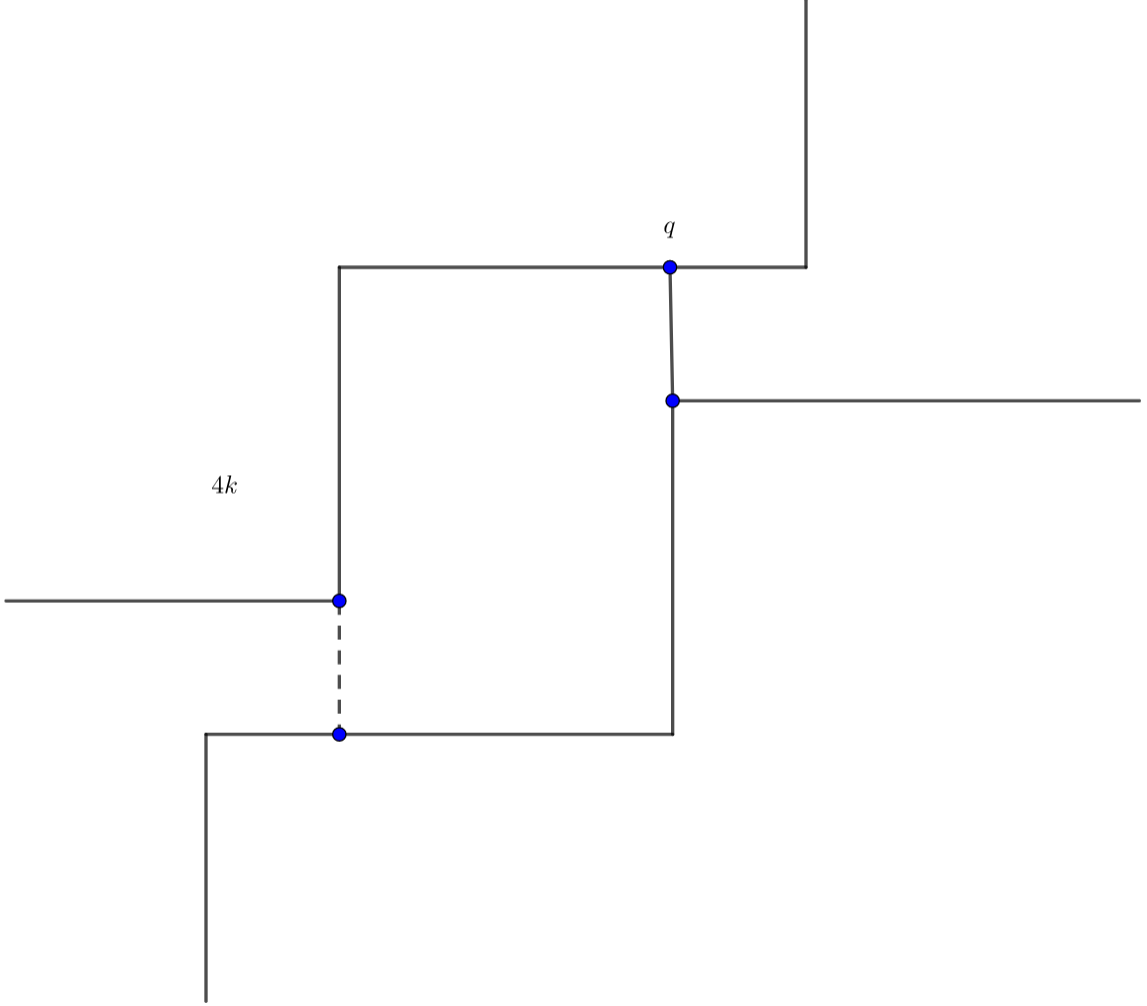
\includegraphics[width=.3 \paperwidth]{./images/EjemplarC1.png}
    \end{subfigure}
    \caption*{Suponemos que el primer corte genera a un corte de tamaño $4k$.}
  \end{figure}
  De lo anterior tenemos $4k - 3 + 1 = 4k - 2 = 4k' + 2$.\newline
  
\end{frame}

\begin{frame}{El problema.} %%Otra forma (más corta) de poner el título a la diapositiva
  \framesubtitle{¿Cuántas lámparas son necesarias para iluminar?} %%Subtítulo de la diapositiva (opcional)
  Otro posibles caso es
  \begin{figure}
    \centering
    \begin{subfigure}[b]{0.25\paperwidth}
      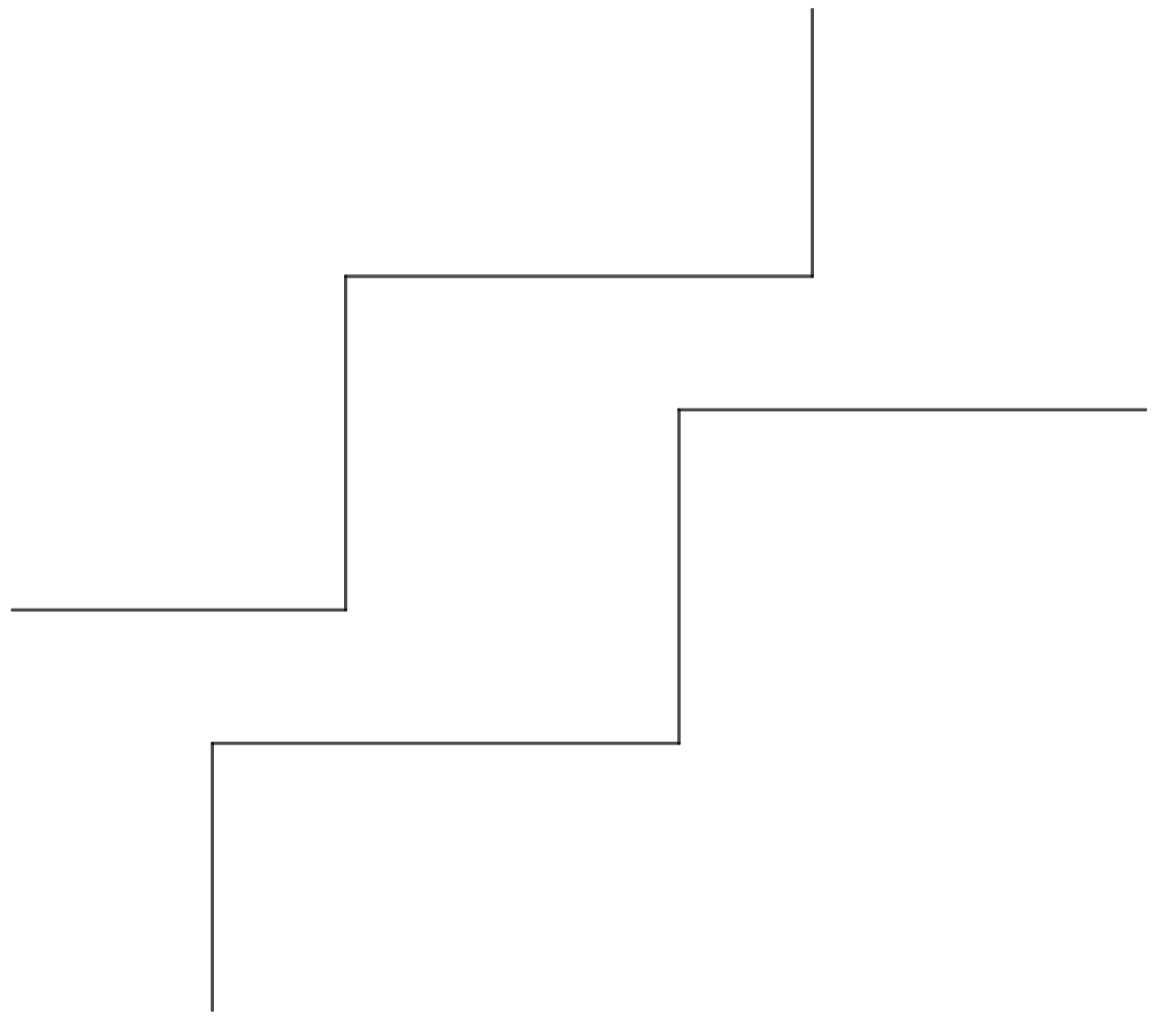
\includegraphics[width=.3 \paperwidth]{./images/Ejemplar.png}
    \end{subfigure}
    \begin{subfigure}[b]{0.25\paperwidth}
      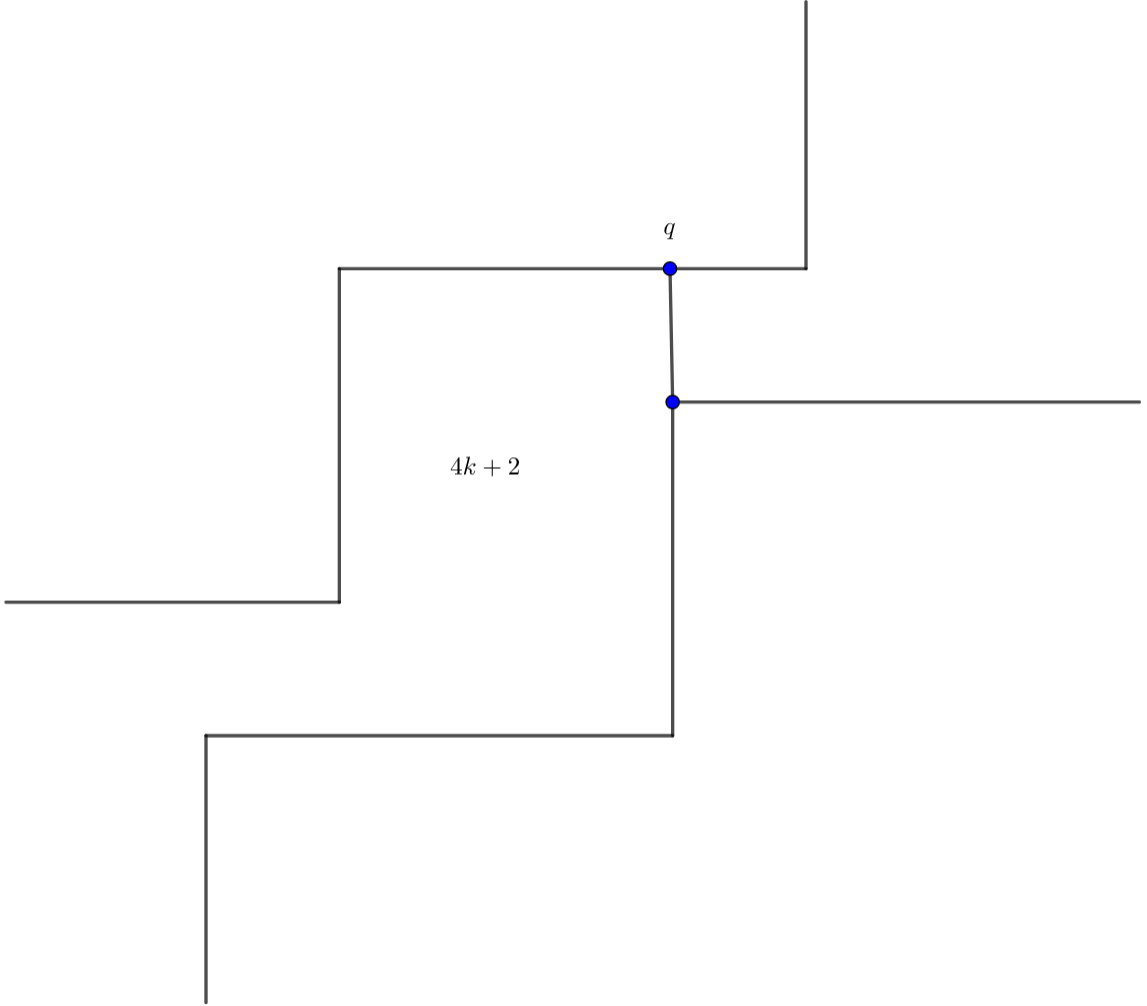
\includegraphics[width=.3 \paperwidth]{./images/EjemplarC2.png}
    \end{subfigure}
    \begin{subfigure}[b]{0.25\paperwidth}
      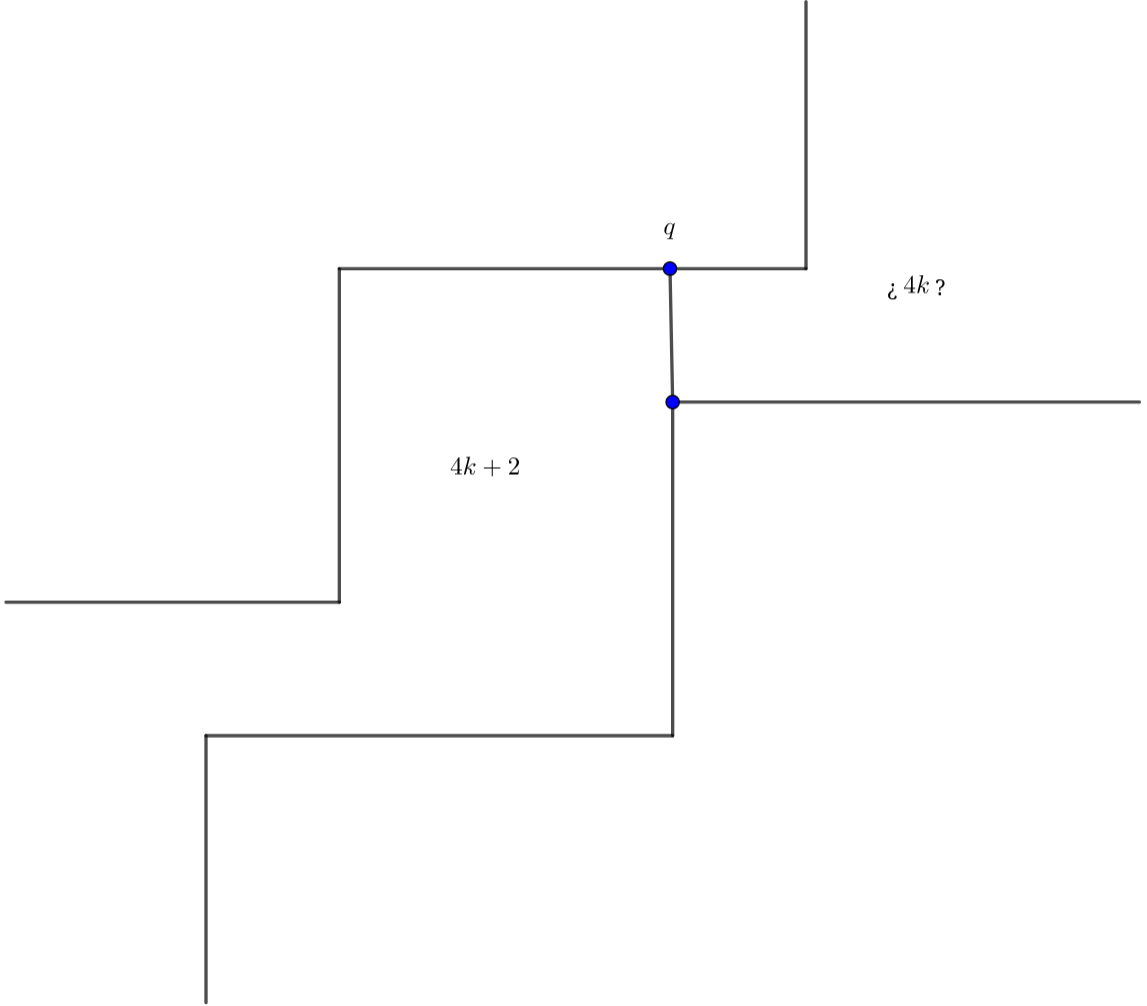
\includegraphics[width=.3 \paperwidth]{./images/EjemplarC2(4k + 2).png}
    \end{subfigure}
    \caption*{Suponemos que ambos cortes generan polígonos de tamaño $4k$.}
  \end{figure}
  De lo anterior tenemos
  \[(4k + 2 - 1) + (4k' - 1) - 1 = 4(k + k') - 1 = 4k'' - 1 \:\: !!!\]
  \newline
  
\end{frame}

\begin{frame}{El problema.} %%Otra forma (más corta) de poner el título a la diapositiva
  \framesubtitle{¿Cuántas lámparas son necesarias para iluminar?} %%Subtítulo de la diapositiva (opcional)
  Para el caso (2) basta extender $e$ y $f'$ hasta que se intersecten y obtenemos un polígno de $n - 4$ vértices
  tal que por inducción se puede iluminar con $\lfloor \frac{n - 4}{4} \rfloor$ lámparas. Por tanto terminamos. \hfill $\square$
  \begin{figure}
    \centering
    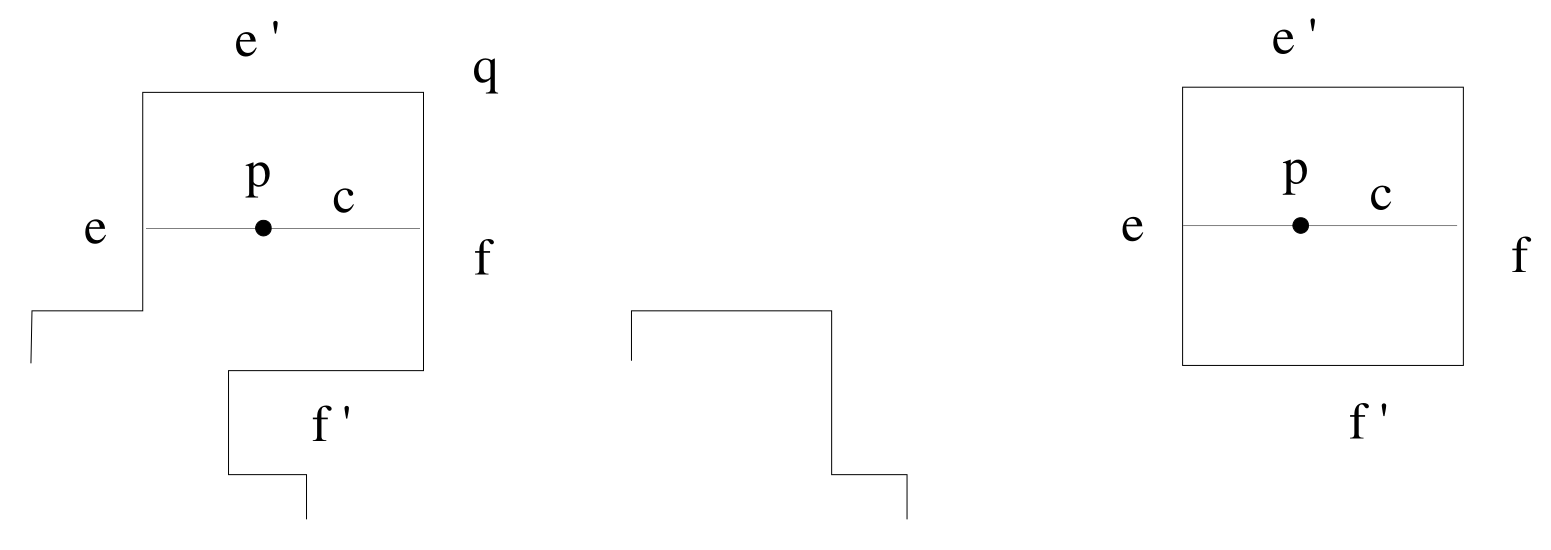
\includegraphics[width=.8 \paperwidth]{./images/Caso2.png}
    \caption*{Bosquejo del punto 2.}
  \end{figure}
\end{frame}


\section{El problema de los Tres Reflectores.} %%Otra sección
\subsection{Colocando reflectores.}
% Teorema
\begin{frame}
    \frametitle{El problema.}    
    \begin{teorema} %%Uso del "environment" definido al inicio del documento.
      Sean $\alpha_1, \alpha_2, \alpha_3$ tres ángulos tales que
      \[\alpha_1 + \alpha_2 + \alpha_3 = \pi\]
      y sea $P$ un polígono convexo. Entonces siempre podemos colocar tres reflectores
      de tamaño a lo más $\alpha_1, \alpha_2, \alpha_3$ con ápices sobre vértices de $P$
      de manera que $P$ quede iluminado, y no coloquemos más de un reflector sobre cada
      vértice de $P$.
    \end{teorema}
\end{frame}

% Demostración:
\begin{frame}
    \frametitle{Prueba.}    
    Es fácil ver que un triángulo cumple con el teorema. Supongamos $P$ un polígono convexo con al menos $4$
    vértices.\newline

    Supongamos que $\alpha_1 \leq \alpha_2 \leq \alpha_3 \Rightarrow \alpha_2 < \frac{\pi}{2}$.  Además, cómo
    $P$ tiene al menos $4$ vértices entonces al menos uno de los ángulos generados por sus vértices es mayor
    o igual que $\frac{\pi}{2}$. Sea $T$ un triángulo cuyos ángulos sean $\alpha_1, \alpha_2,$ y $\alpha_3$
    tal que:
    \begin{enumerate}
    \item El vértice de $T$ de tamaño $\alpha_2$ está colocado sobre un vértice $v$ de $P$ que genera un ángulo
      mayor o igual a $\alpha_2$.
    \item Los otros dos vértices de $T$ están colocados sobre dos puntos $x, y$ en la frontera de $P$.
    \end{enumerate}
    Supongamos que $x,y$ pertenecen a aristas distintas en $P$.
\end{frame}

\begin{frame}
  \frametitle{Prueba.}
  Análicemos dos posibles casos:
  \begin{enumerate}
  \item $u \not= w$. Coloquemos un reflector $f_1$ sobre $u$ iluminando la zona angular
    determinada por $v, u, x$ y otro, $f_3$ sobre $w$ iluminado la zona angular
    determinada por $v, w, y$. Como $f_1$ y $f_3$ no están en el interior de $C$, los
    angulos de iluminación de $f_1$ y $f_3$ son a lo más, $\alpha_1$ y $\alpha_2$ respectivamente.
  \item $u = w$. Sea $T'$ el triángulo determinado por el segmento que une a $x$ con
    $y$, y las tangentes a $C$ en estos puntos. El ángulo generado en el vértice
    $z$ de $T'$  que no está sobre $C$ es $\pi - 2\alpha_2$. Nótese que $z$ pertenece al interior
    del triángulo $T''$ con vértices $x, y, u$ y por tanto el ángulo de $T''$ en $u$ es
    menor que $\pi - 2\alpha_2$. Como $\alpha \leq \alpha_2 \leq \alpha_3 \leq \pi - 2\alpha_2 \leq (\pi - (\alpha_1 + \alpha_2)) = \alpha_3$.
    Por tanto colocando un reflector de tamaño a lo más $\alpha_3$ en u iluminamos P.
  \end{enumerate}
\end{frame}


{\setbeamertemplate{background}{

\includegraphics[width=\the\paperwidth,height=\the\paperheight]{images/White.png}}

\begin{frame}
  \frametitle{Caso 1.}
  \begin{figure}
    \centering
    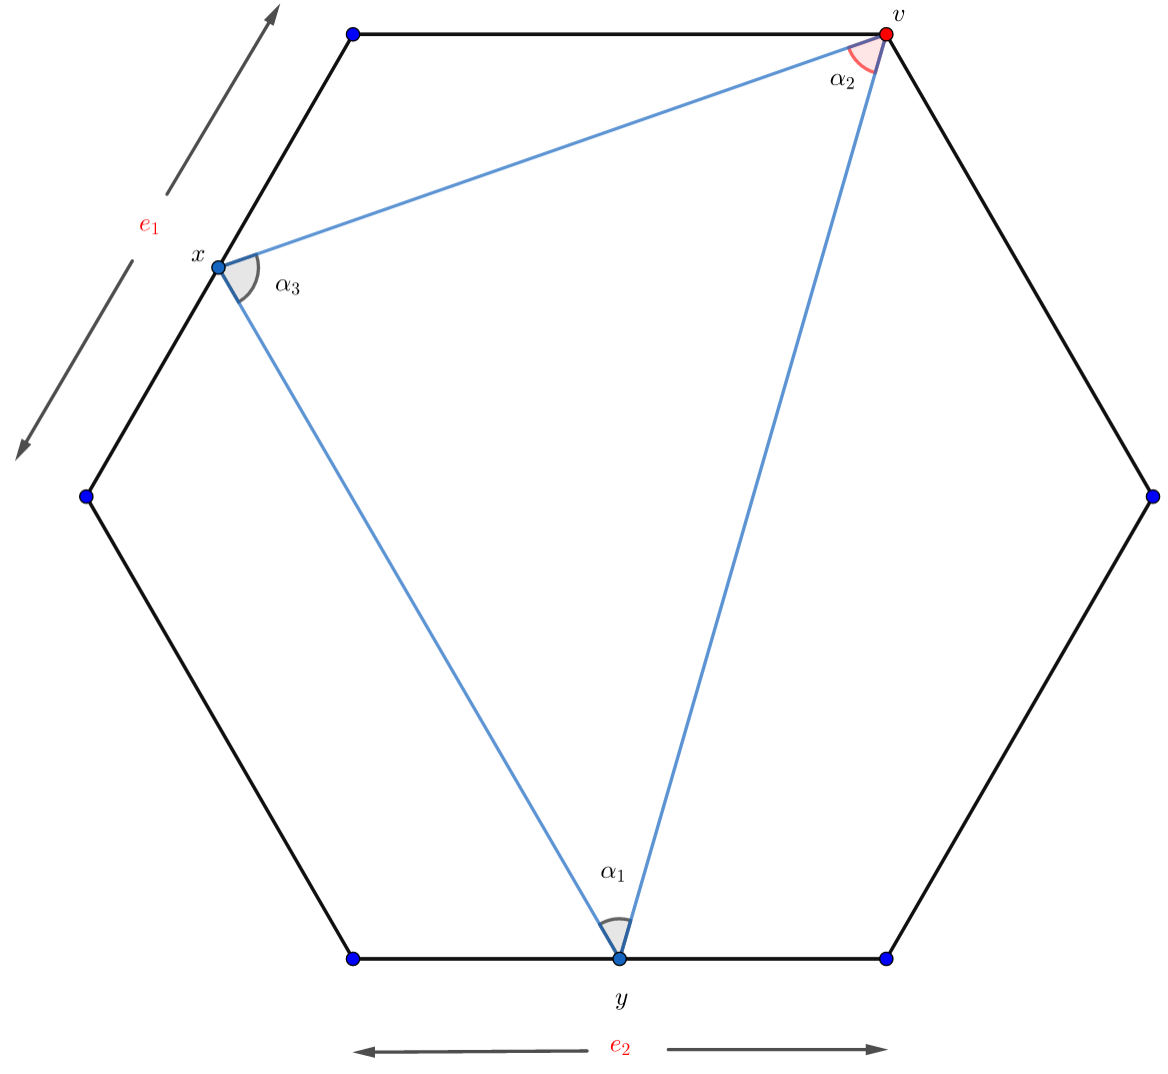
\includegraphics[width=.50 \paperwidth]{./images/Bosquejo1.png}
    %\caption*{.}
  \end{figure}
\end{frame}

\begin{frame}
  %\frametitle{Prueba.}
  \begin{figure}
    \centering
    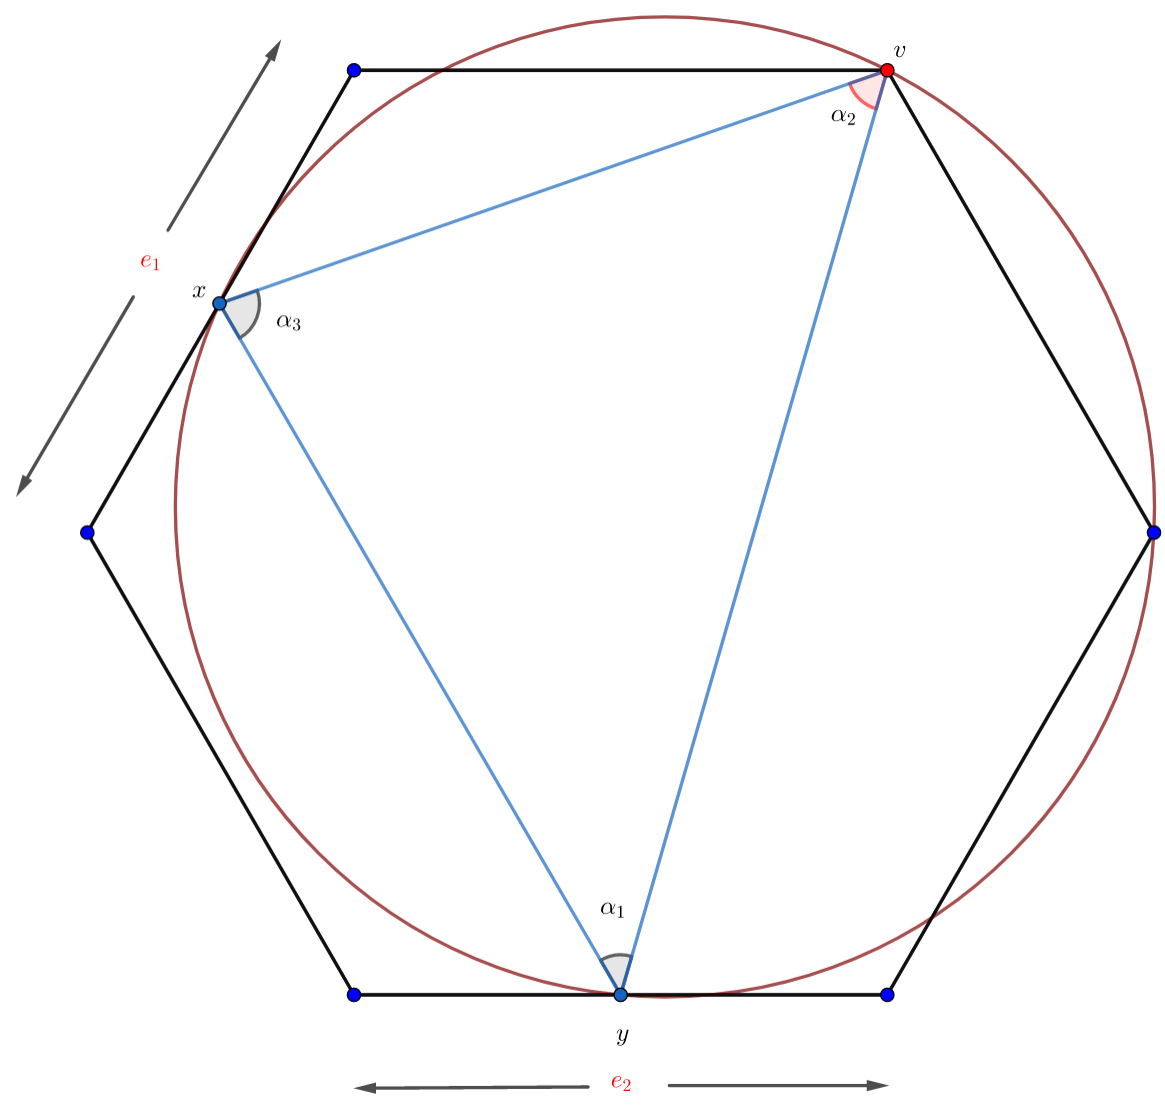
\includegraphics[width=.65 \paperwidth]{./images/Bosquejo2.png}
    %\caption*{.}
  \end{figure}
\end{frame}

\begin{frame}
  %\frametitle{Prueba.}
  \begin{figure}
    \centering
    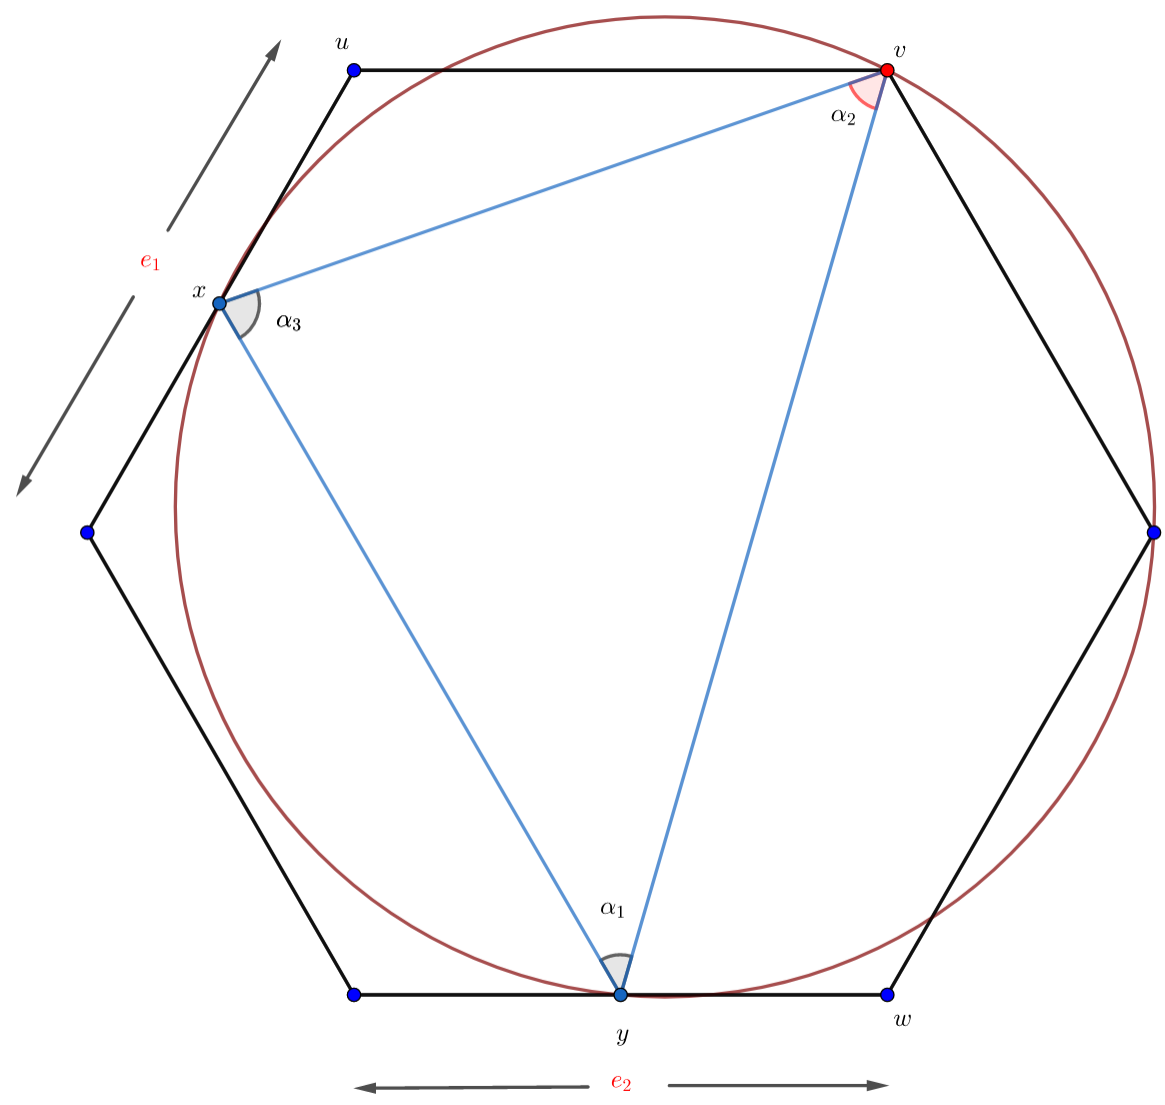
\includegraphics[width=.65 \paperwidth]{./images/Bosquejo3.png}
    %\caption*{.}
  \end{figure}
\end{frame}

\begin{frame}
  %\frametitle{Prueba.}
  \begin{figure}
    \centering
    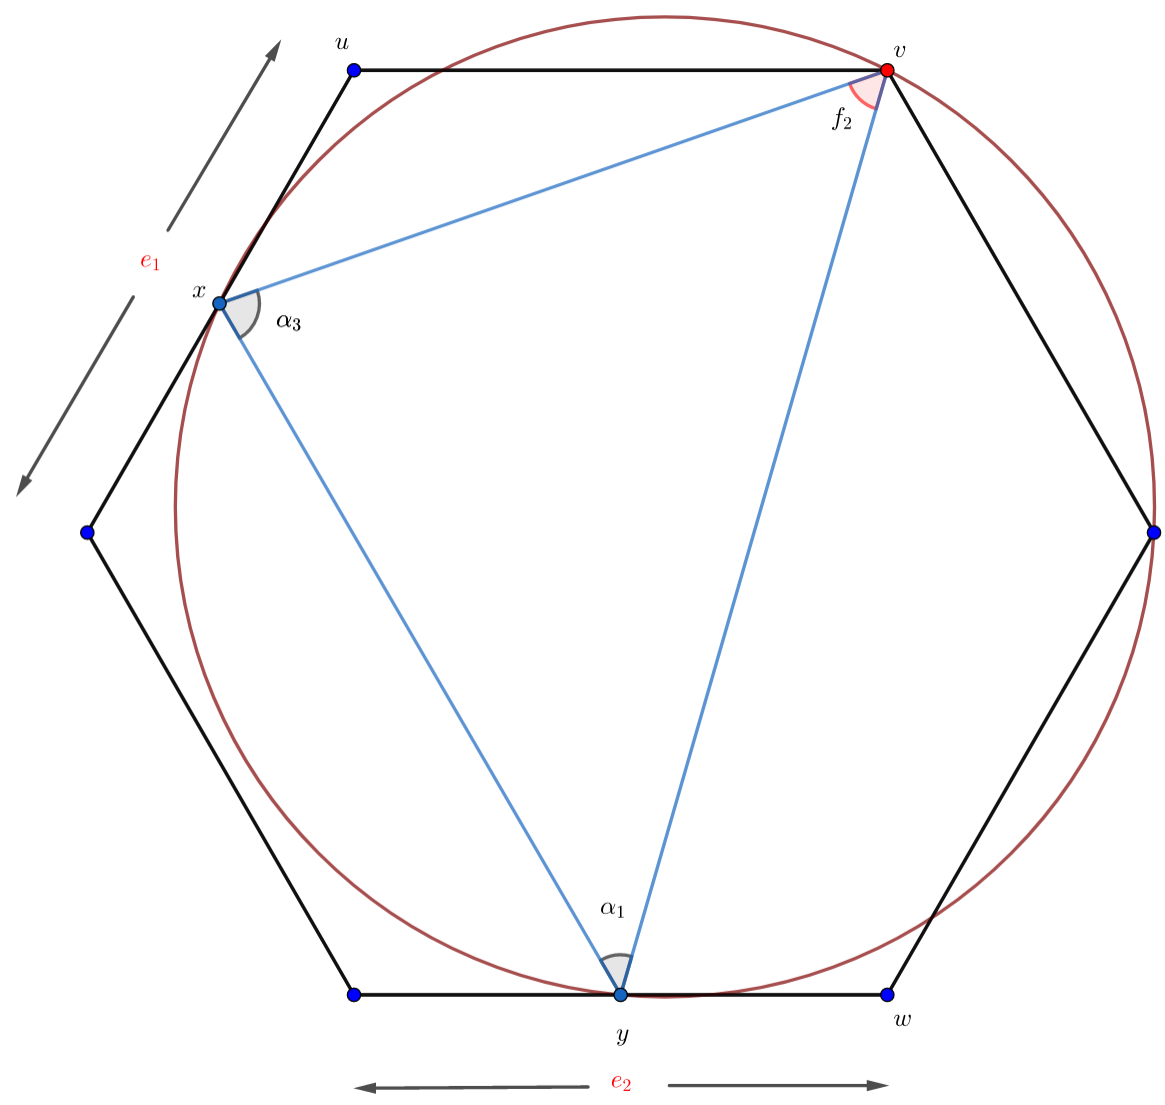
\includegraphics[width=.65 \paperwidth]{./images/Bosquejo4.png}
    %\caption*{.}
  \end{figure}
\end{frame}

\begin{frame}
  %\frametitle{Prueba.}
  \begin{figure}
    \centering
    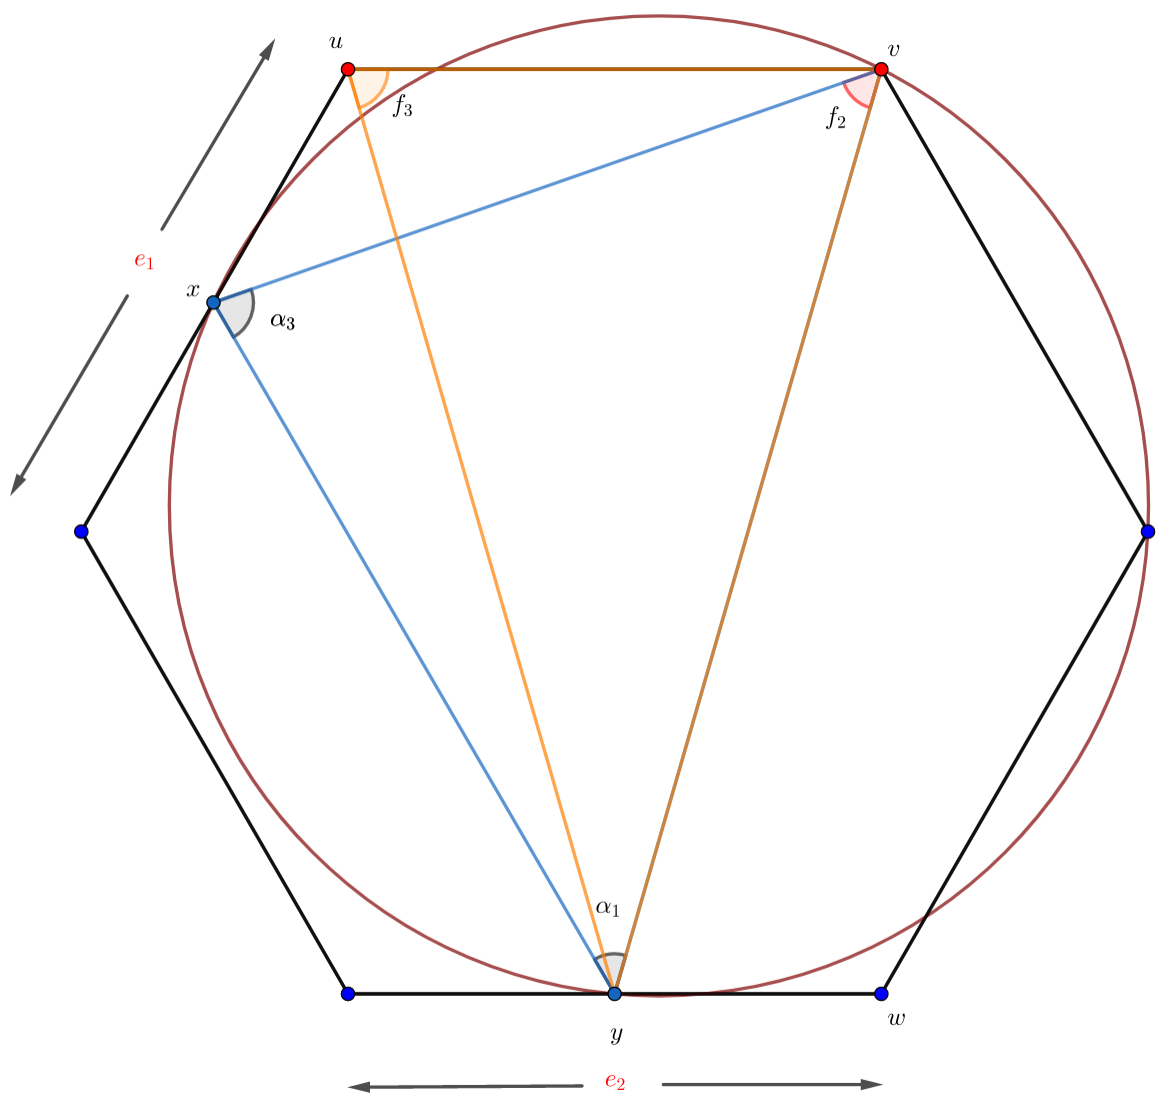
\includegraphics[width=.65 \paperwidth]{./images/Bosquejo5.png}
    %\caption*{.}
  \end{figure}
\end{frame}

\begin{frame}
  %\frametitle{Prueba.}
  \begin{figure}
    \centering
    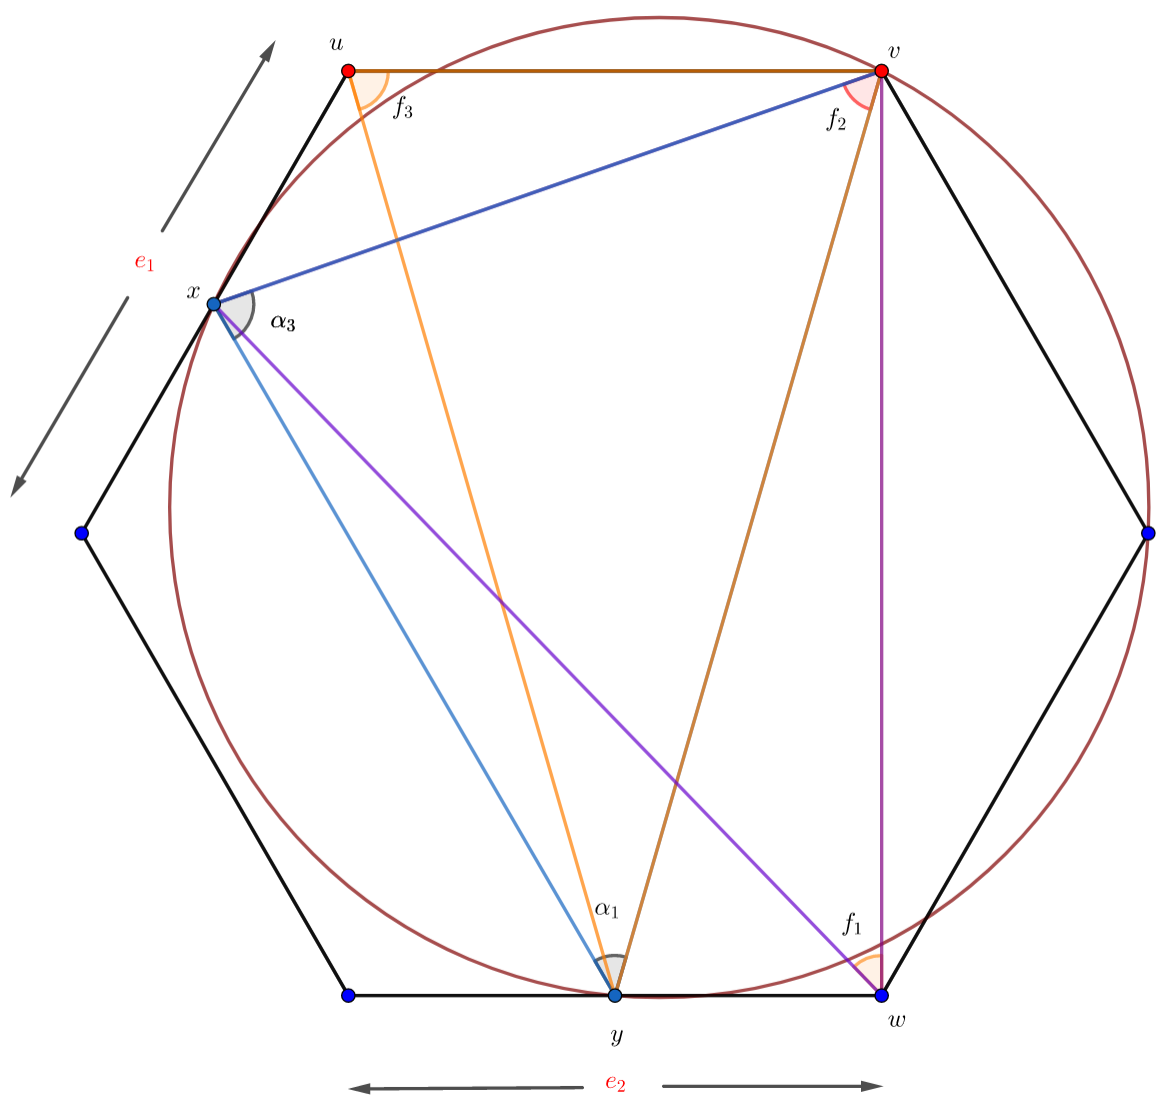
\includegraphics[width=.65 \paperwidth]{./images/Bosquejo6.png}
    %\caption*{.}
  \end{figure}
\end{frame} 

\begin{frame}
  %\frametitle{Prueba.}
  \begin{figure}
    \centering
    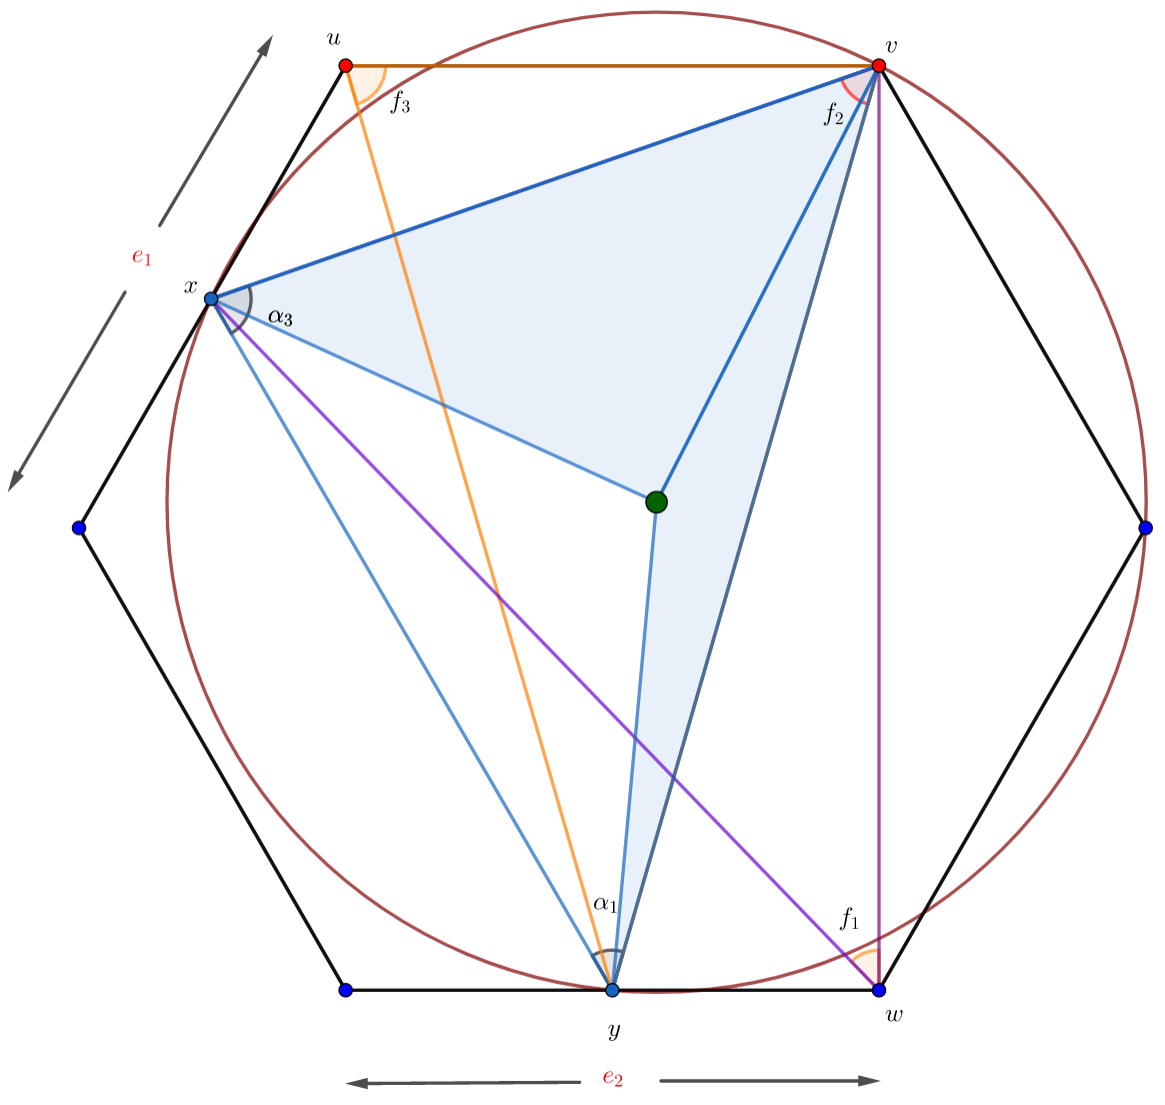
\includegraphics[width=.65 \paperwidth]{./images/Bosquejo7.png}
    %\caption*{.}
  \end{figure}
\end{frame} 

\begin{frame}
  %\frametitle{Prueba.}
  \begin{figure}
    \centering
    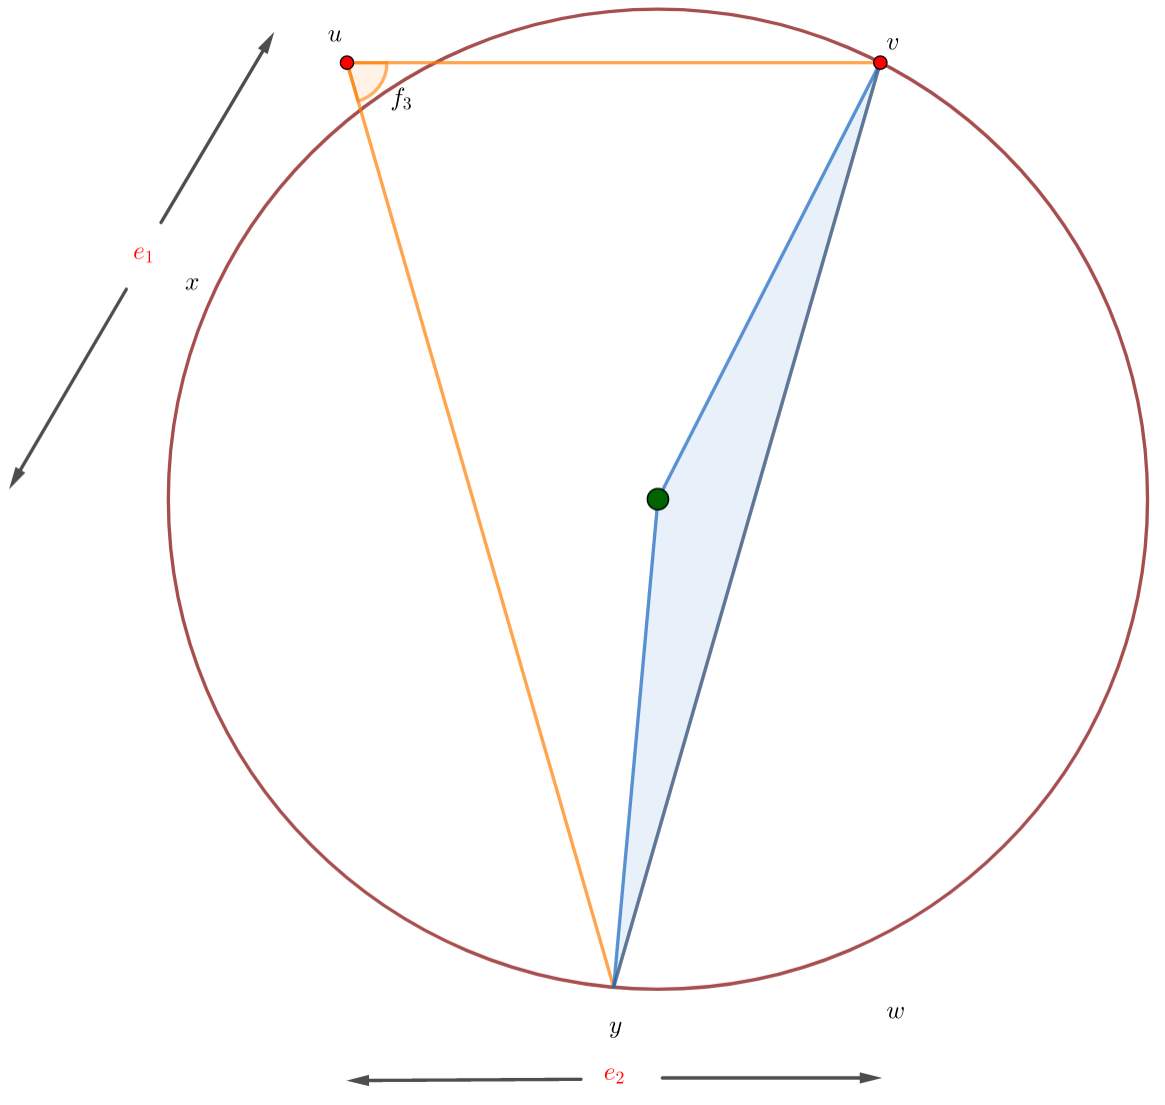
\includegraphics[width=.65 \paperwidth]{./images/Bosquejo8.png}
    %\caption*{.}
  \end{figure}
\end{frame} 

\begin{frame}
  %\frametitle{Prueba.}
  \begin{figure}
    \centering
    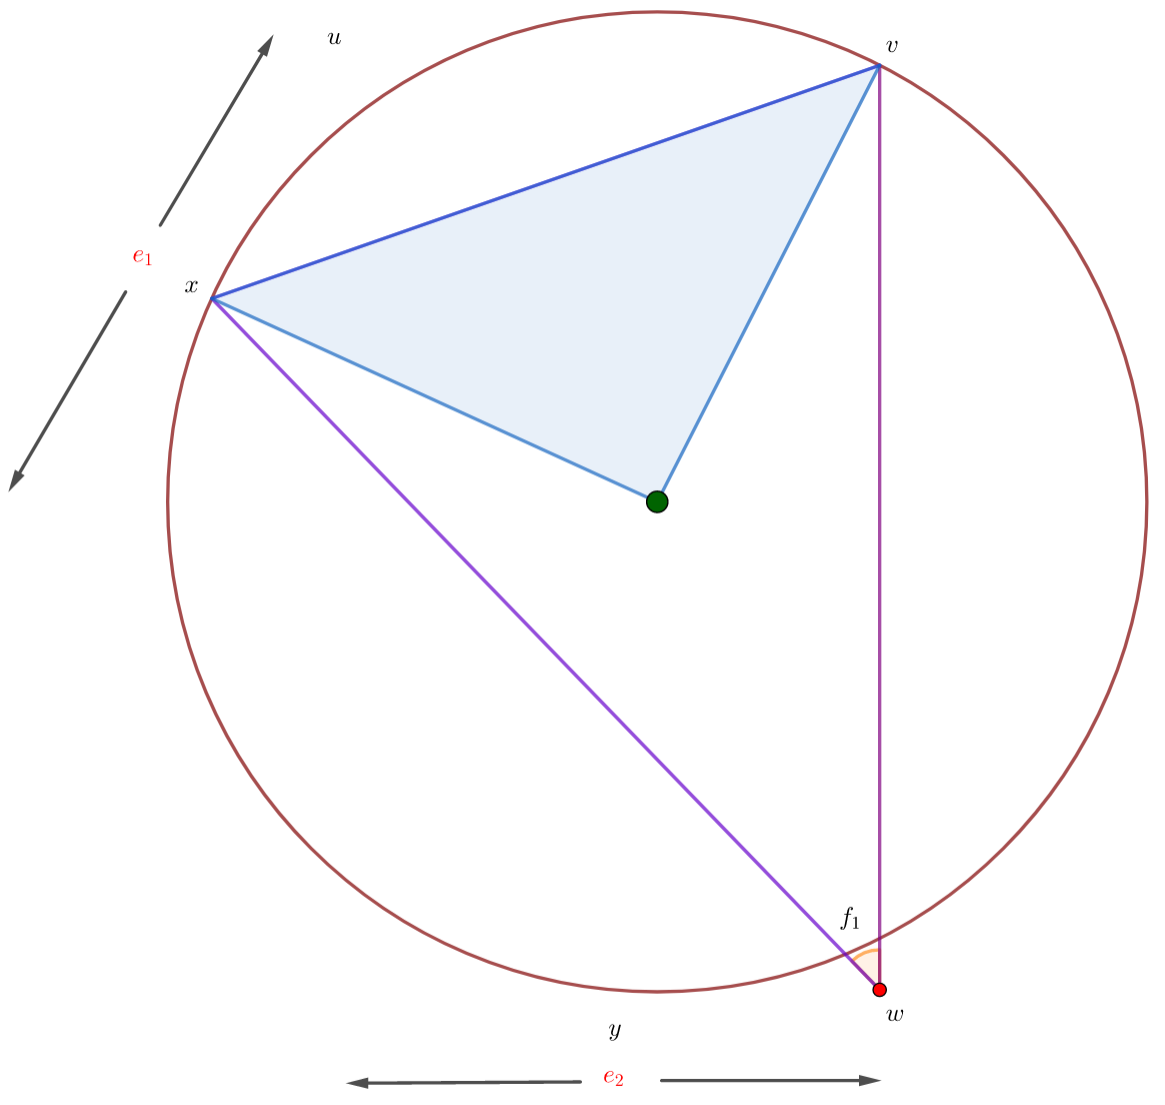
\includegraphics[width=.65 \paperwidth]{./images/Bosquejo9.png}
    %\caption*{.}
  \end{figure}
\end{frame} 

\begin{frame}
  %\frametitle{Prueba.}
  \begin{figure}
    \centering
    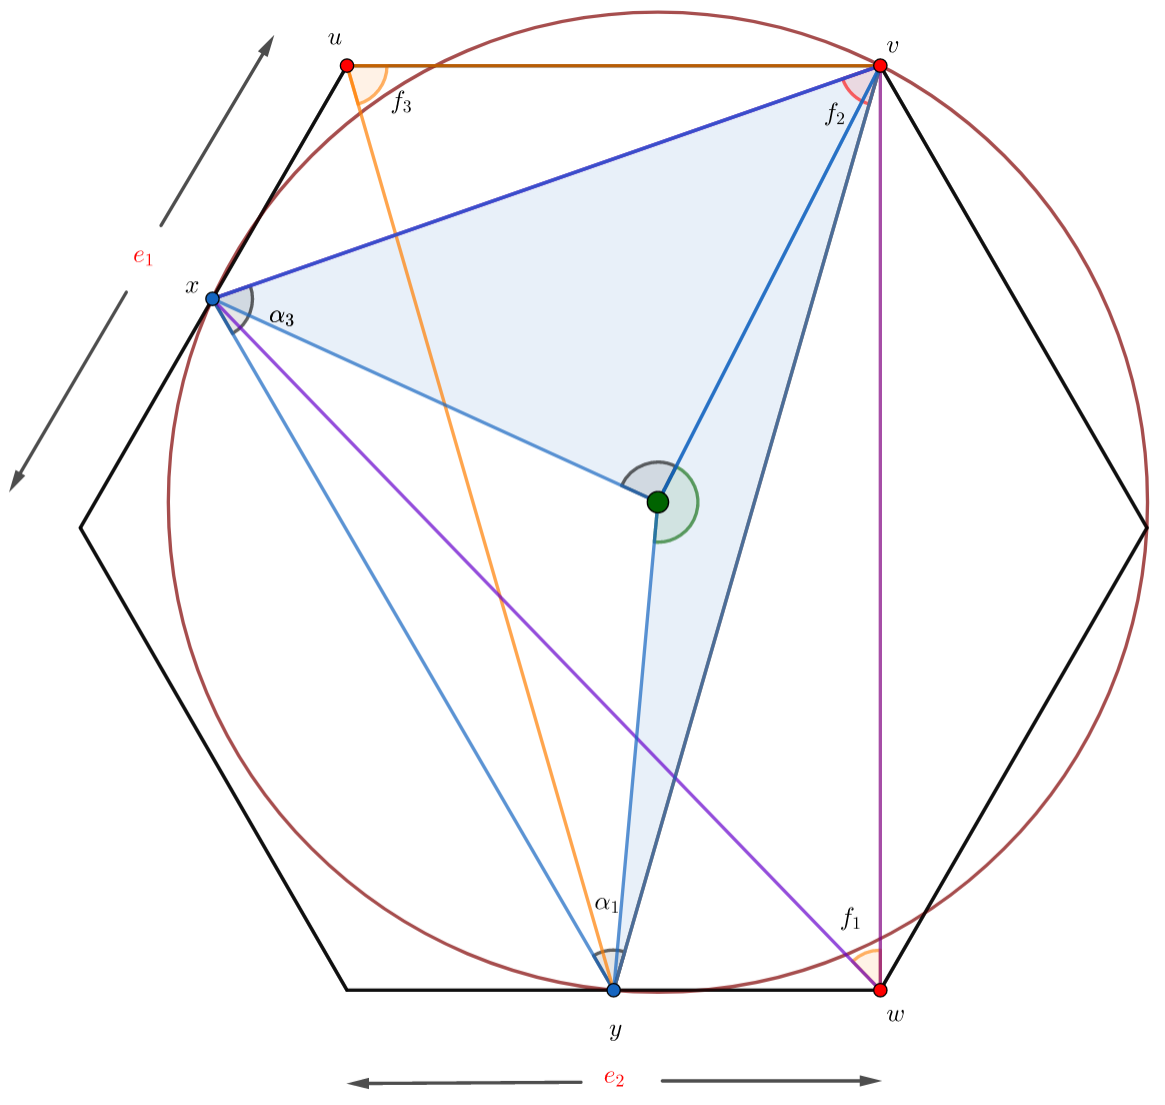
\includegraphics[width=.65 \paperwidth]{./images/Bosquejo10.png}
    %\caption*{.}
  \end{figure}
\end{frame} 

\begin{frame}
  \frametitle{Cuentas ...}
  Primero observemos que
  \begin{eqnarray*}
    \sphericalangle vox &=& 2 \alpha_1\\
    \sphericalangle voy &=& 2 \alpha_3
  \end{eqnarray*}
  Luego, tenemos que
 \begin{eqnarray*}
    f_1 &=& \frac{2\alpha_1 - \sphericalangle x'}{2}\\
    f_3 &=& \frac{2\alpha_3 - \sphericalangle y'}{2}
  \end{eqnarray*}
 En partícular, se cumple que
 \begin{eqnarray*}
    f_1 + f_3 &=& \frac{2\alpha_1 - \sphericalangle x'}{2} +  \frac{2\alpha_3 - \sphericalangle y'}{2}\\
              &=& \alpha_1 + \alpha_3 - \frac{\sphericalangle x' + \sphericalangle y'}{2}
 \end{eqnarray*}

 .\newline

 .
\end{frame} 


\begin{frame}
  %\frametitle{Prueba.}
  \begin{figure}
    \centering
    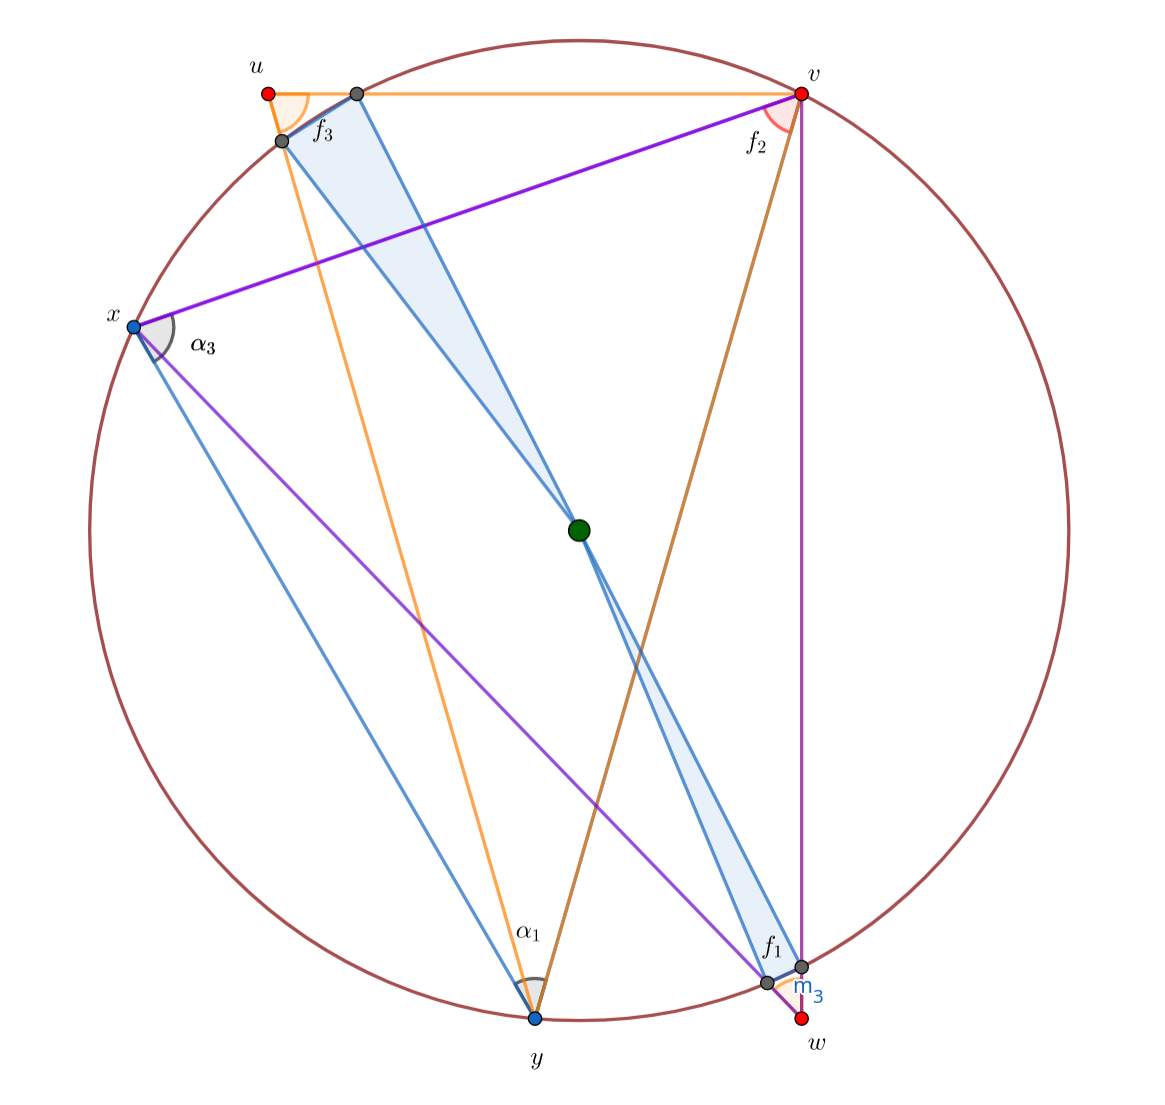
\includegraphics[width=.65 \paperwidth]{./images/Bosquejo11.png}
    %\caption*{.}
  \end{figure}
\end{frame} 

\begin{frame}
  %\frametitle{Prueba.}
  \begin{figure}
    \centering
    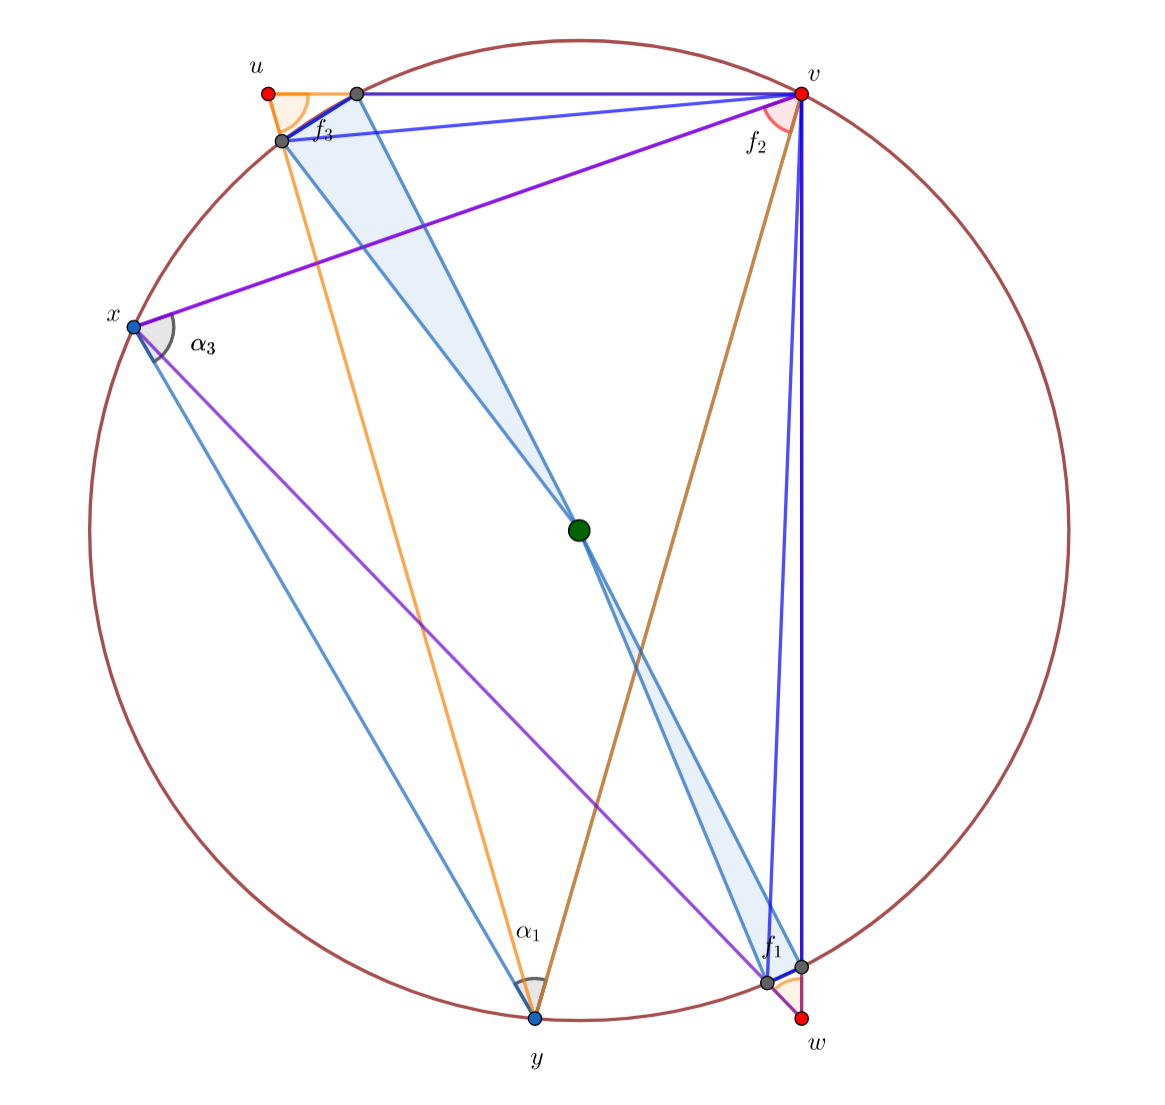
\includegraphics[width=.65 \paperwidth]{./images/Bosquejo12.png}
    %\caption*{.}
  \end{figure}
\end{frame} 

\begin{frame}
  %\frametitle{Prueba.}
  \begin{figure}
    \centering
    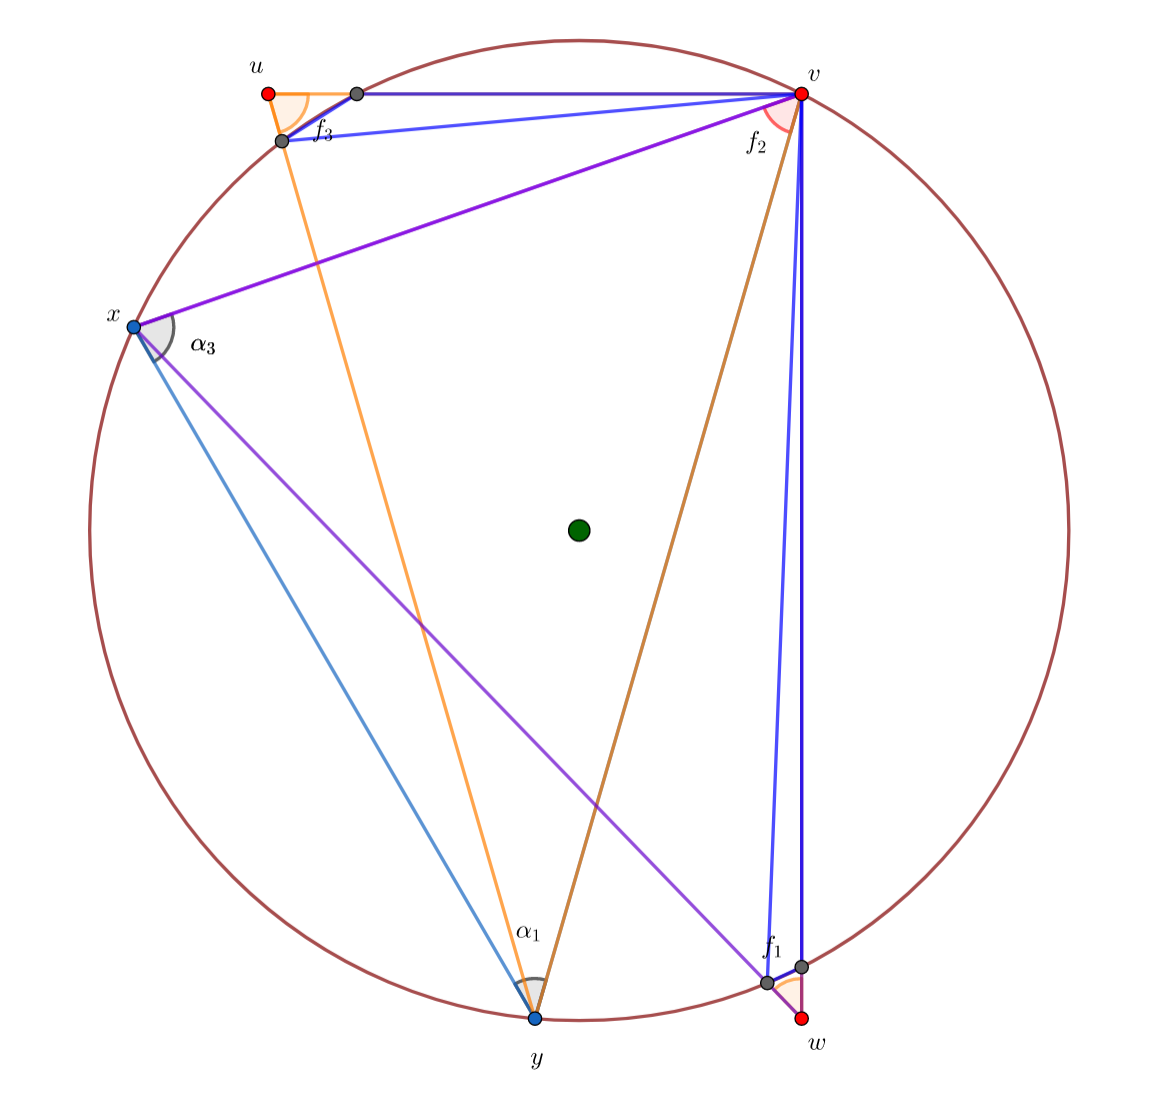
\includegraphics[width=.65 \paperwidth]{./images/Bosquejo13.png}
    %\caption*{.}
  \end{figure}
\end{frame} 

\begin{frame}
  %\frametitle{Prueba.}
  \begin{figure}
    \centering
    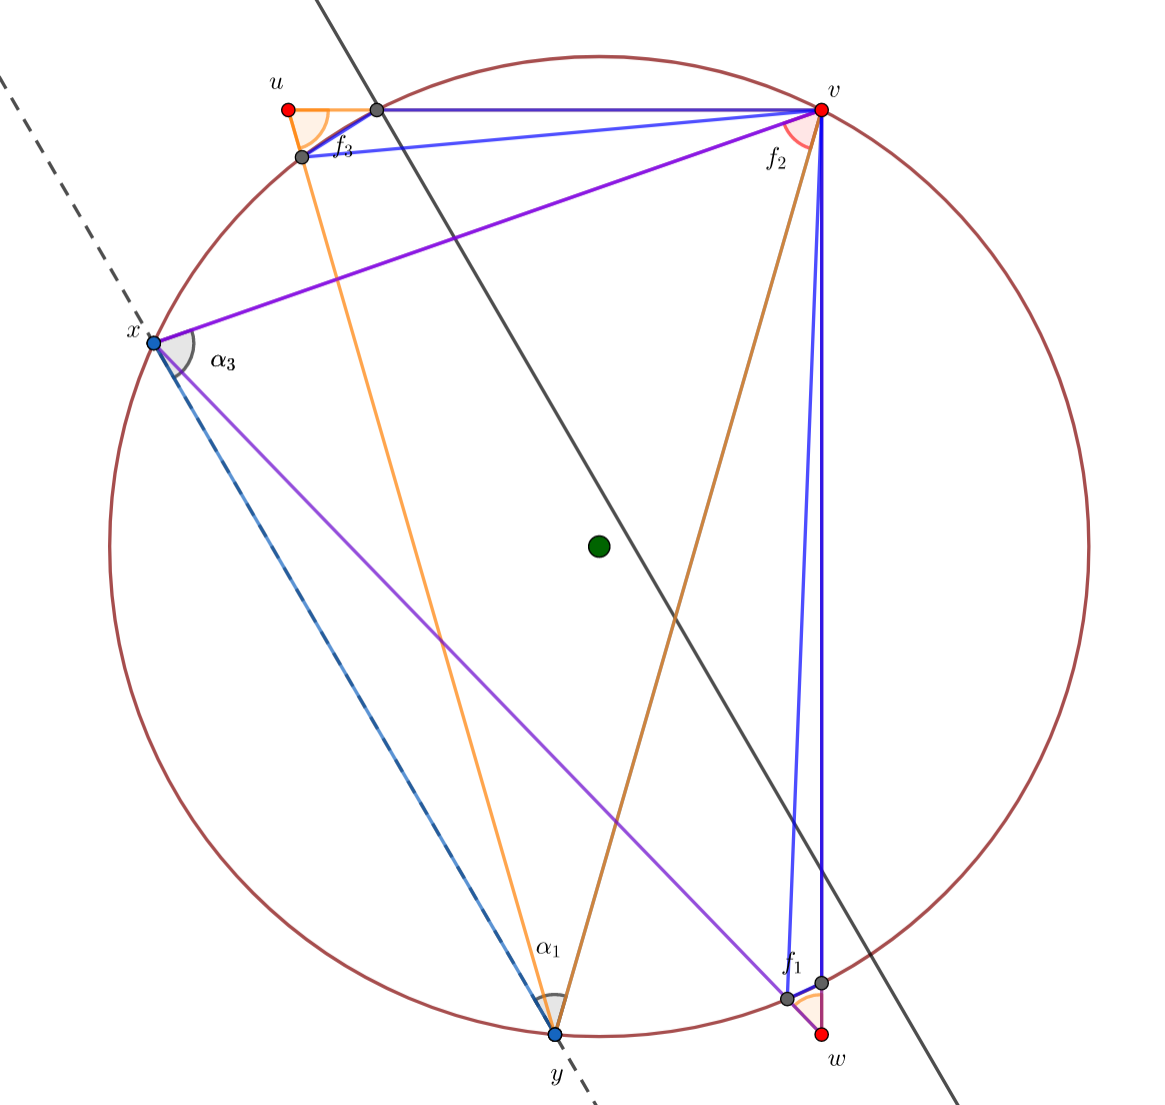
\includegraphics[width=.65 \paperwidth]{./images/Bosquejo14.png}
    %\caption*{.}
  \end{figure}
\end{frame}

\begin{frame}
  %\frametitle{Prueba.}
  \begin{figure}
    \centering
    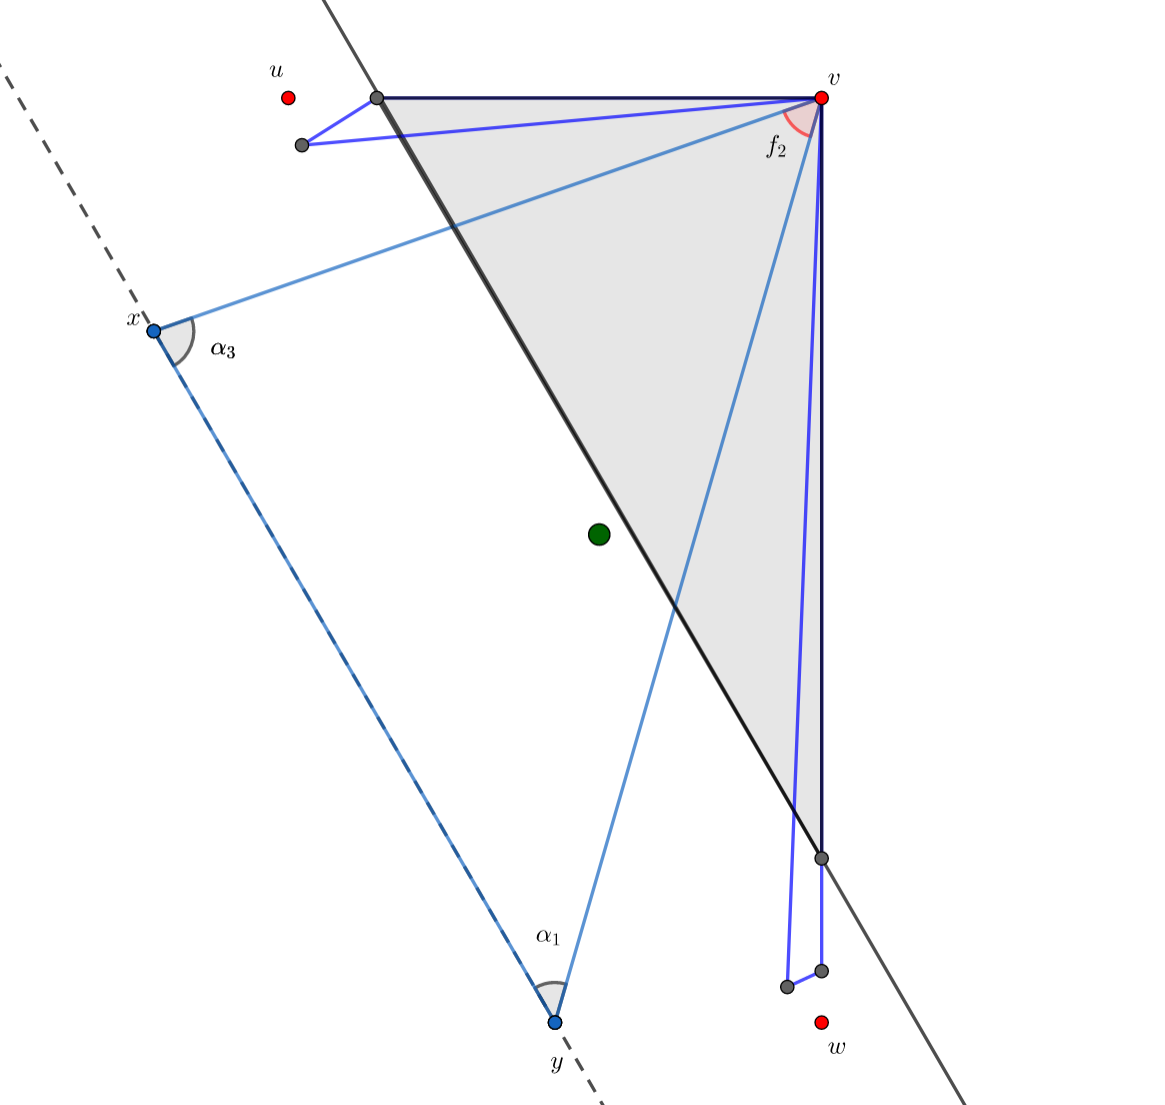
\includegraphics[width=.65 \paperwidth]{./images/Bosquejo15.png}
    %\caption*{.}
  \end{figure}
\end{frame}

\begin{frame}
  %\frametitle{Prueba.}
  \begin{figure}
    \centering
    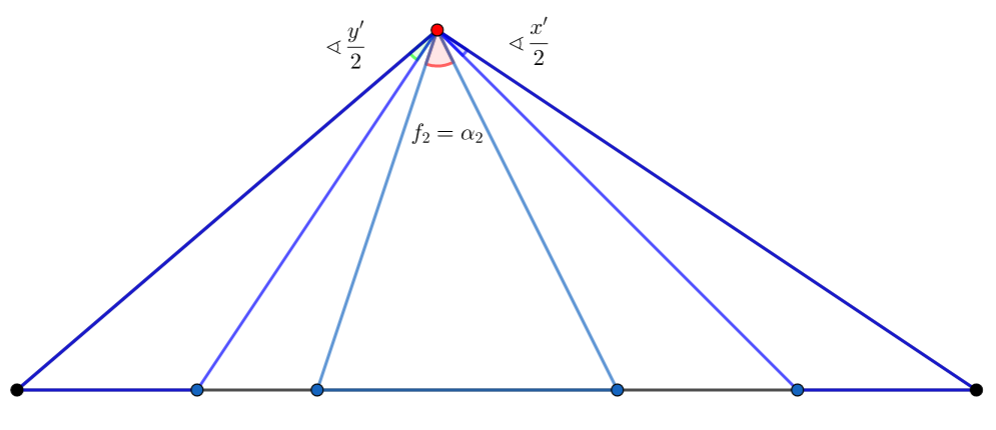
\includegraphics[width=.65 \paperwidth]{./images/D1.png}
    %\caption*{.}
  \end{figure}
\end{frame}

\begin{frame}
  %\frametitle{Prueba.}
  \begin{figure}
    \centering
    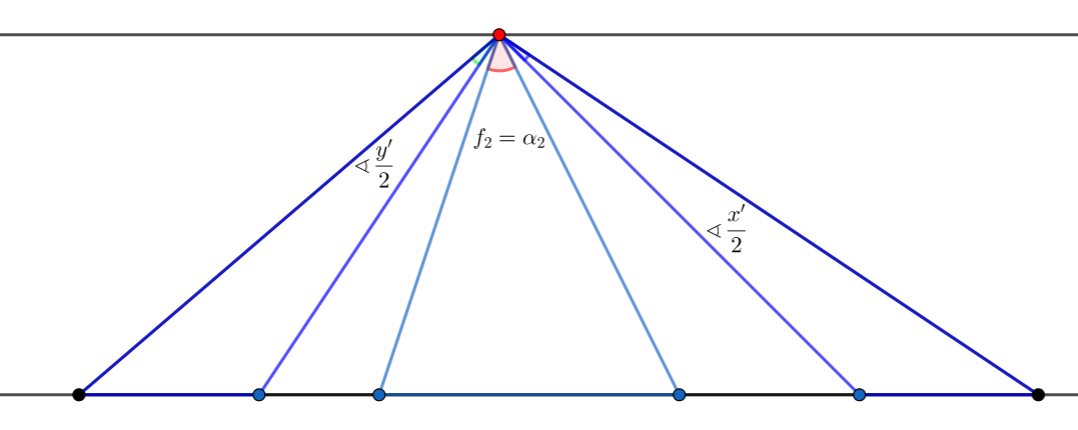
\includegraphics[width=.65 \paperwidth]{./images/D2.png}
    %\caption*{.}
  \end{figure}
\end{frame}

\begin{frame}
  %\frametitle{Prueba.}
  \begin{figure}
    \centering
    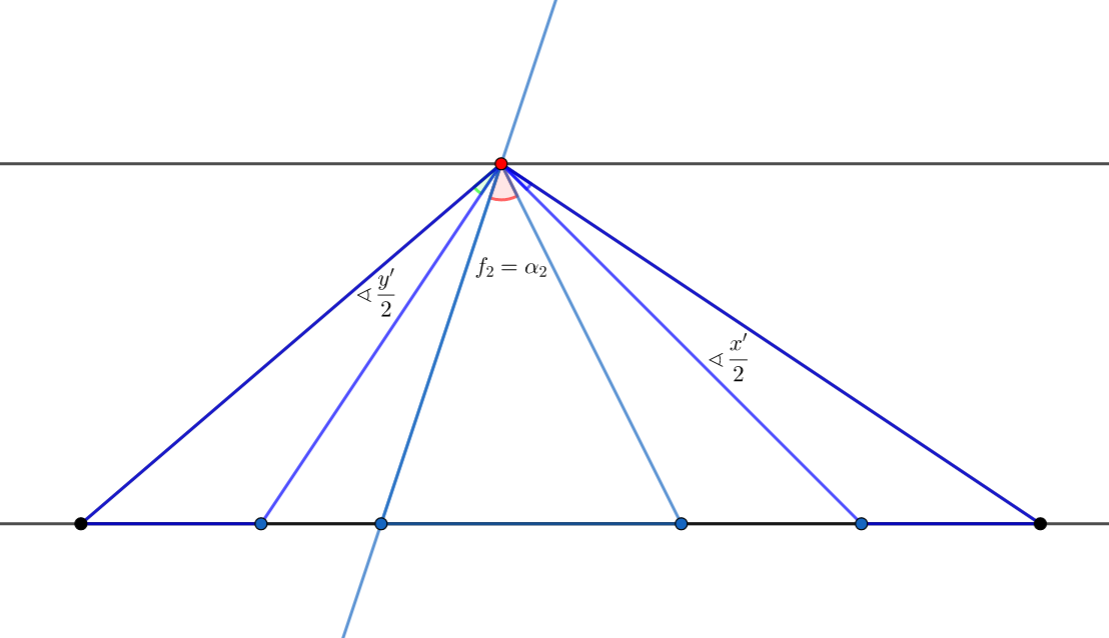
\includegraphics[width=.65 \paperwidth]{./images/D3.png}
    %\caption*{.}
  \end{figure}
\end{frame}

\begin{frame}
  %\frametitle{Prueba.}
  \begin{figure}
    \centering
    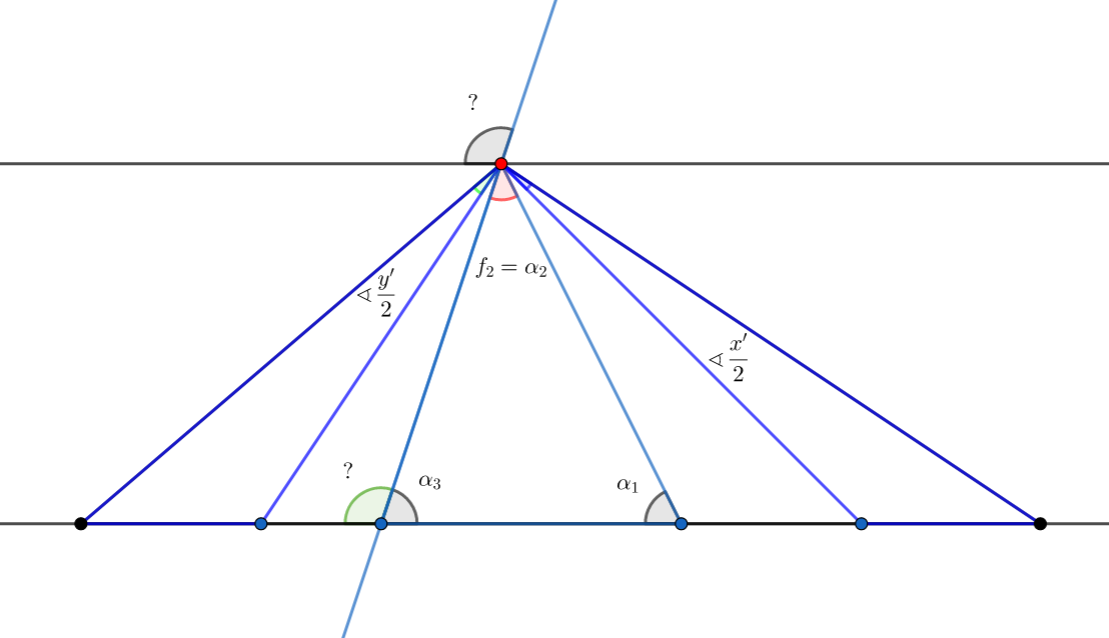
\includegraphics[width=.65 \paperwidth]{./images/D4.png}
    %\caption*{.}
  \end{figure}
\end{frame}

\begin{frame}
  %\frametitle{Prueba.}
  \begin{figure}
    \centering
    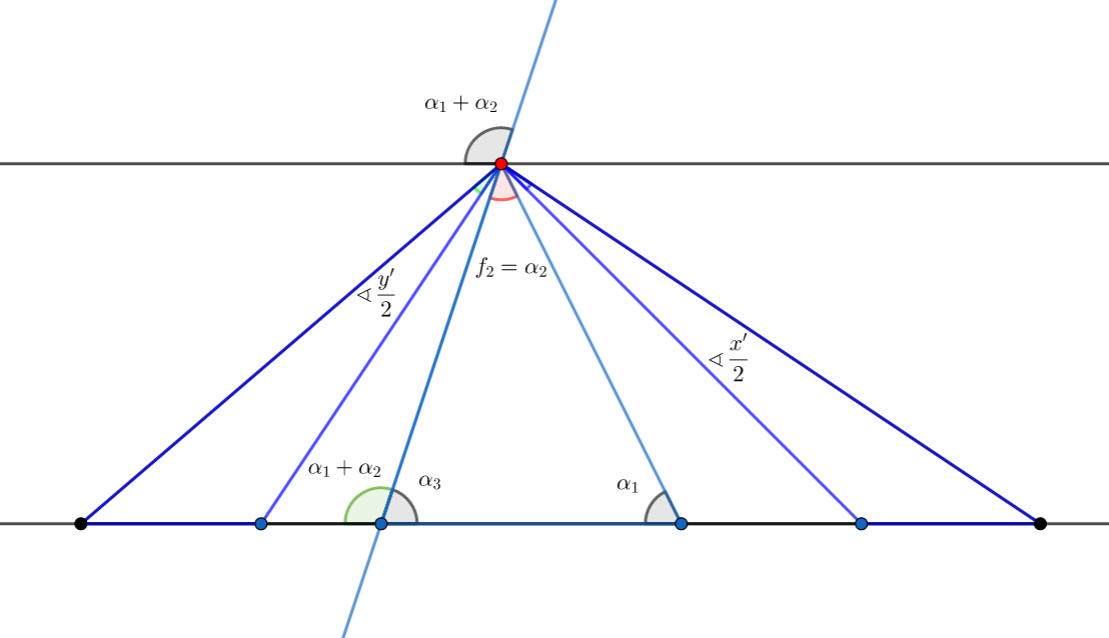
\includegraphics[width=.65 \paperwidth]{./images/D5.png}
    %\caption*{.}
  \end{figure}
\end{frame}

\begin{frame}
  \frametitle{Cuentas ...}
  Esto implica que
  \begin{eqnarray*}
    \sphericalangle \frac{x'}{2} &<& \alpha_1\\
    \sphericalangle \frac{y'}{2} &<& \alpha_3
  \end{eqnarray*}
  Luego, tenemos que
 \begin{eqnarray*}
   f_1 + f_3 &=& \alpha_1 + \alpha_3 - \frac{\sphericalangle x' + \sphericalangle y'}{2}\\
             &\leq& \alpha_1 + \alpha_3
 \end{eqnarray*}
 Por lo anterior, tenemos que
 \begin{eqnarray*}
   f_1 + f_2 + f_3 &\leq& \alpha_1 + \alpha_ 2+ \alpha_3.
 \end{eqnarray*}
\end{frame} 

\begin{frame}
  \frametitle{Caso 2.}
  \begin{figure}
    \centering
    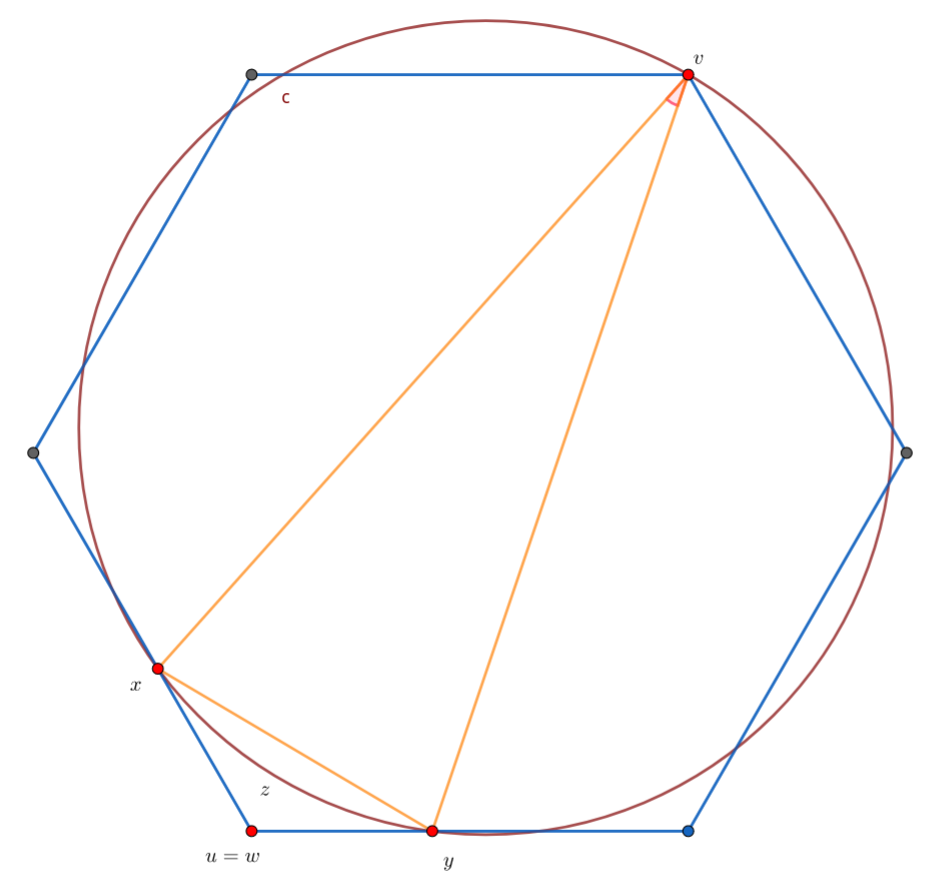
\includegraphics[width=.50 \paperwidth]{./images/Bosquejo16.png}
    %\caption*{.}
  \end{figure}
\end{frame}

\begin{frame}
  %\frametitle{Caso 2.}
  \begin{figure}
    \centering
    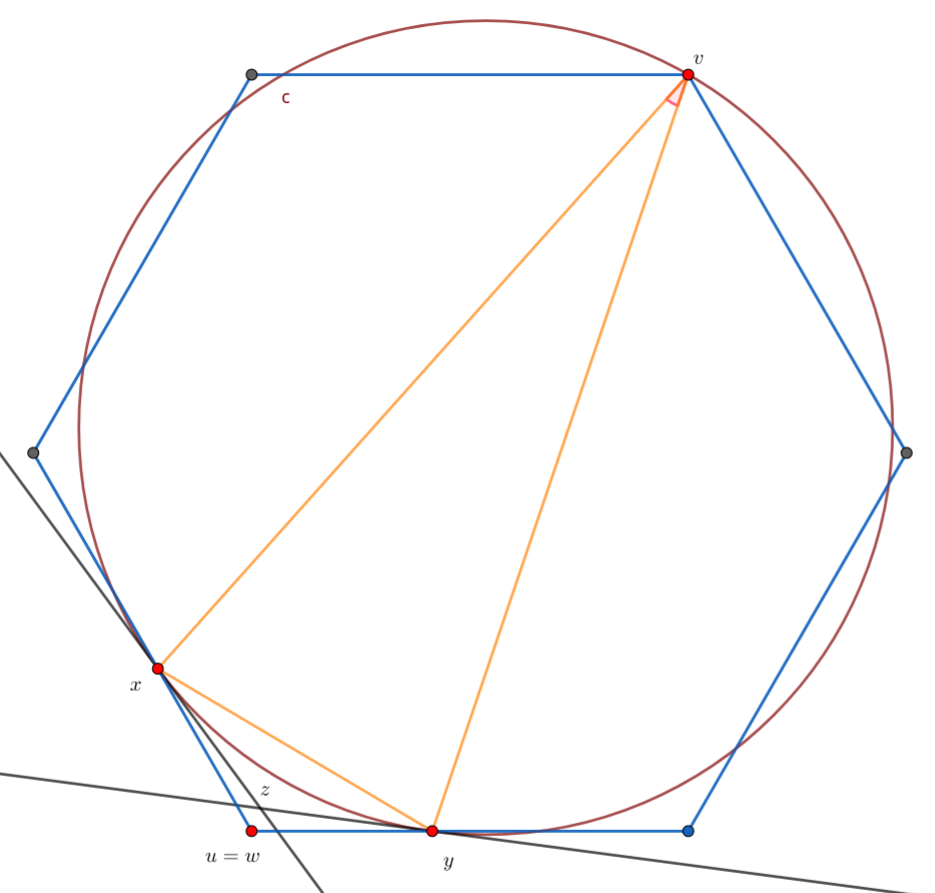
\includegraphics[width=.65 \paperwidth]{./images/Bosquejo17.png}
    %\caption*{.}
  \end{figure}
\end{frame}

\begin{frame}
  %\frametitle{Caso 2.}
  \begin{figure}
    \centering
    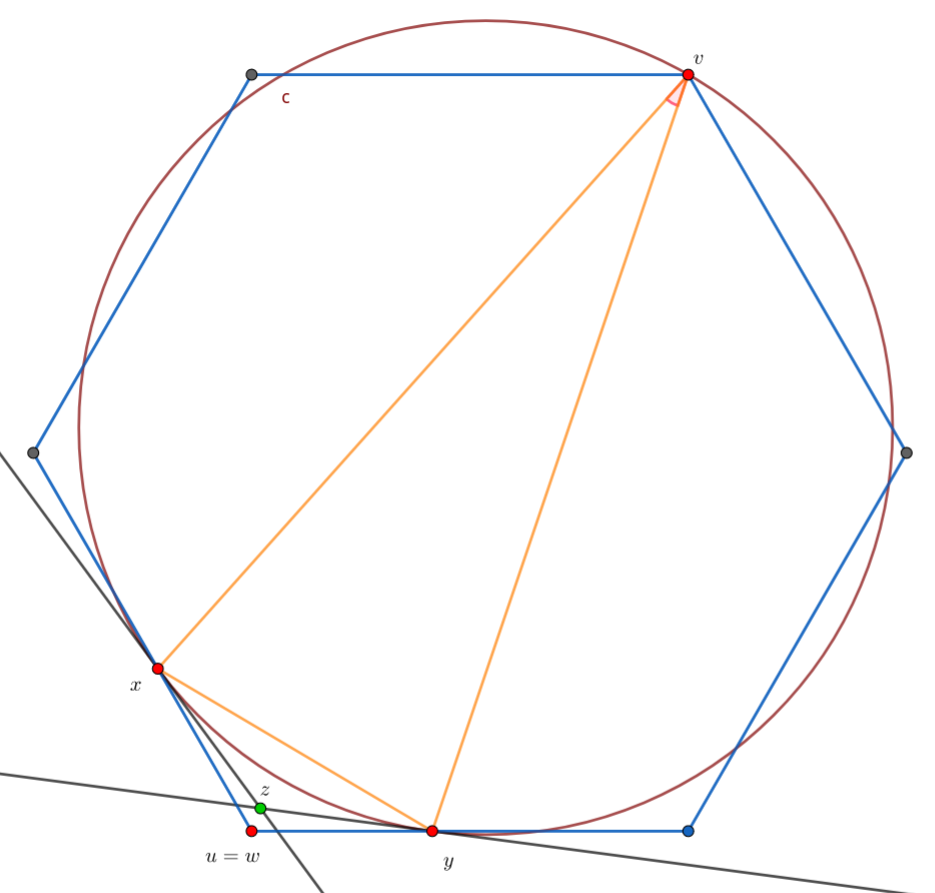
\includegraphics[width=.65 \paperwidth]{./images/Bosquejo18.png}
    %\caption*{.}
  \end{figure}
\end{frame}

\begin{frame}
  %\frametitle{Caso 2.}
  \begin{figure}
    \centering
    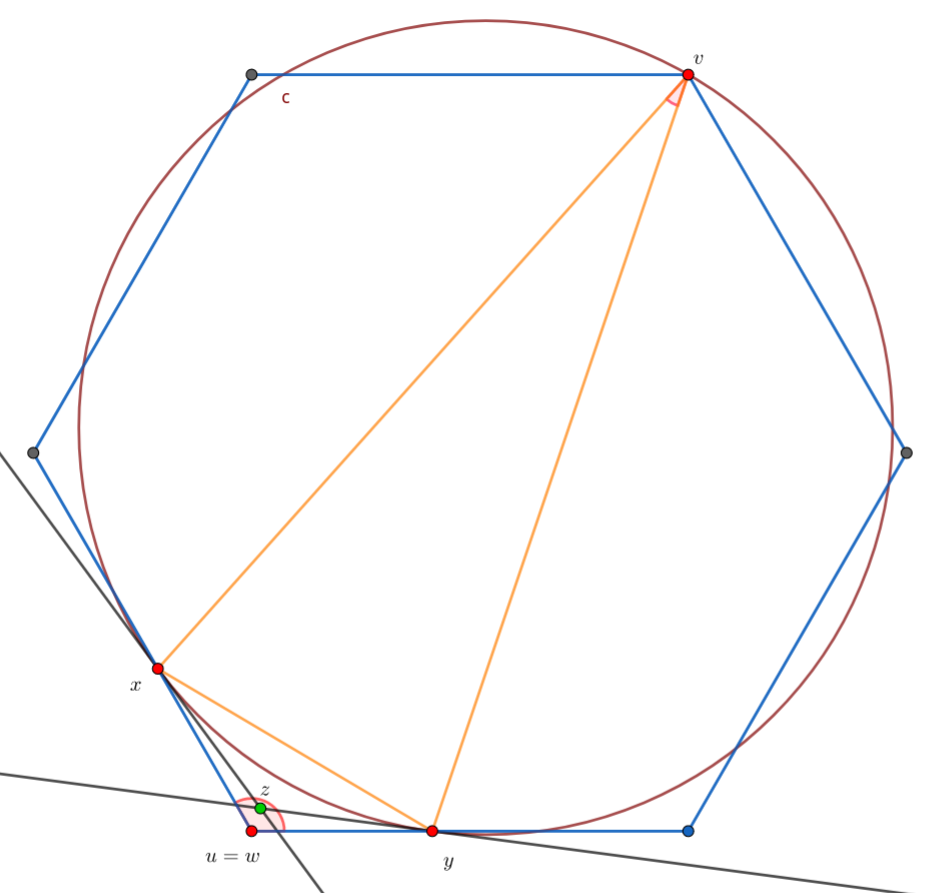
\includegraphics[width=.65 \paperwidth]{./images/Bosquejo19.png}
    %\caption*{.}
  \end{figure}
\end{frame} 

\begin{frame}
  \frametitle{Cuentas ...}
  De lo anterior tenemos que
  \begin{eqnarray*}
    \sphericalangle z &=& \frac{(2\pi - 2\alpha_2) - 2\alpha_2}{2}\\
                      &=& \frac{2\pi - 4\alpha_2}{2}\\
                      &=& \pi - 2\alpha_2\\
    \Rightarrow \sphericalangle w = \alpha_3 &<& \pi - 2\alpha_2\\
    \Rightarrow \alpha_2 + \alpha_3 &<& \pi - \alpha_2\\
    \Rightarrow \alpha_1 + \alpha_2 + \alpha_3 &<& \pi - (\alpha_2 + \alpha_1) \leq \pi.
  \end{eqnarray*}
  \hfill $\square$
\end{frame} 

\input{./05Reflectores}


\section{El número de aristas de visibilidad de un polígono.}
\subsection{Antecedentes.}
% Antecedentes
\begin{frame}
  \frametitle{Antecedentes I.}    
  Sea $P$ un polígono simple con $n$ vértices. Definimos
  \begin{itemize}
  \item $int(P) \rightarrow \#$ aristas estrictamente internas. 
  \item $ext(P) \rightarrow \#$ aristas estrictamente externas.
  \item Vértice interno de $P$ si pertenece al interior de $Conv(P)$.
  \end{itemize}
    \begin{figure}
    \centering
    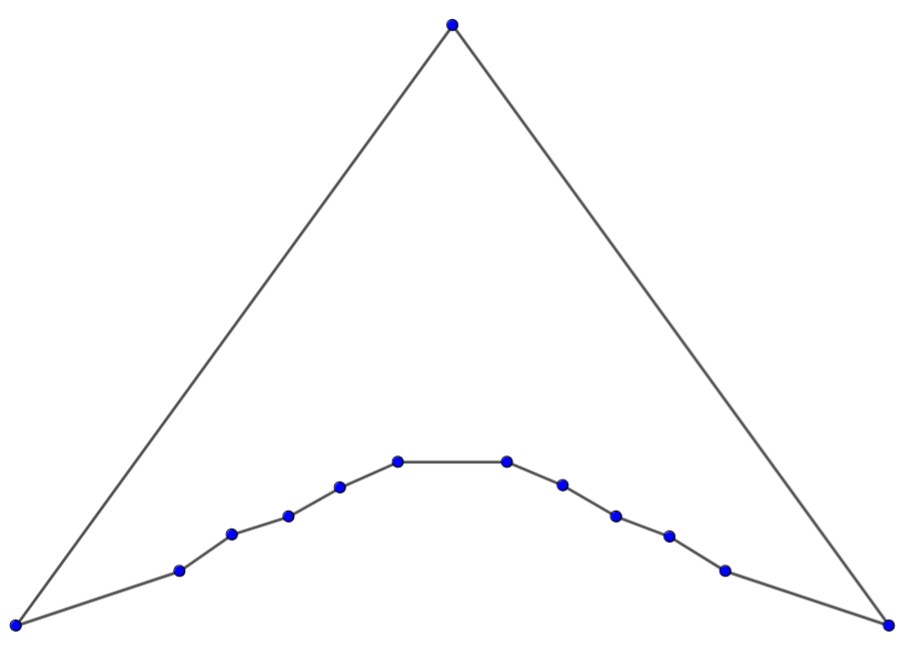
\includegraphics[width=.30 \paperwidth]{./images/Ejemplo1.png}
    \caption*{Polígono.}
  \end{figure}
\end{frame}


\begin{frame}
  \frametitle{Antecedentes I.}    
  Sea $P$ un polígono simple con $n$ vértices. Definimos
  \begin{itemize}
  \item $int(P) \rightarrow \#$ aristas estrictamente internas. 
  \item $ext(P) \rightarrow \#$ aristas estrictamente externas.
  \end{itemize}
    \begin{figure}
    \centering
    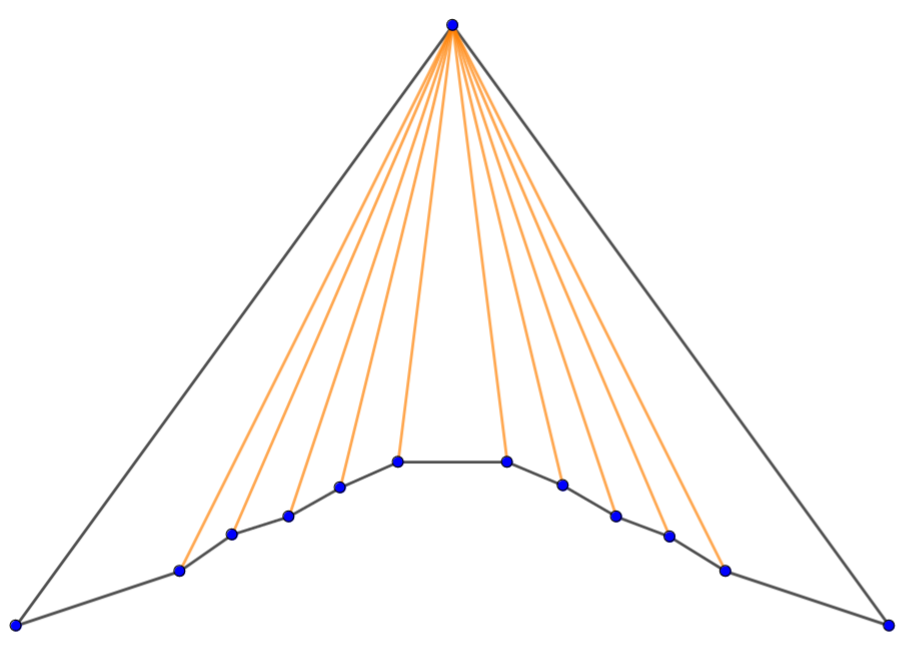
\includegraphics[width=.35 \paperwidth]{./images/Ejemplo2.png}
    \caption*{Algunas aristas extrictamente internas.}
  \end{figure}
\end{frame}

\begin{frame}
  \frametitle{Antecedentes I.}    
  Sea $P$ un polígono simple con $n$ vértices. Definimos
  \begin{itemize}
  \item $int(P) \rightarrow \#$ aristas estrictamente internas. 
  \item $ext(P) \rightarrow \#$ aristas estrictamente externas.
  \end{itemize}
  \begin{figure}
    \centering
    \includegraphics[width=.35 \paperwidth]{./images/Ejemplo3.png}
    \caption*{Algunas aristas extrictamente externas.}
  \end{figure}
\end{frame}

\begin{frame}
  \frametitle{Antecedentes II.}    
  \begin{lema}
    Sea $P$ un polígono de $n$ vértices, con $k$ vértices internos. Entonces \[ext(P) \geq k.\]
  \end{lema}
  \textbf{Dem.} Analicemos dos posibles casos:\newline
  \textit{Caso 1.} $p \in V_P$ tal que es interno y sus vecinos son parte de $V_{Conv(P)}$. Entonces
  existe una $e \in E_{Conv(P)}$ que es estrictamente externa.
  \begin{figure}
    \centering
    \includegraphics[width=.15 \paperwidth]{./images/Caso01.png}
    %\caption*{Caso 1.}
  \end{figure}
\end{frame}

\begin{frame}
  \frametitle{Antecedentes II.}    
  \begin{lema}
    Sea $P$ un polígono de $n$ vértices, con $k$ vértices internos. Entonces \[ext(P) \geq k.\]
  \end{lema}
  \textbf{Dem.} Analicemos dos posibles casos:\newline
  \textit{Caso 2.} Hay al menos $2$ vértices vecinos internos. Entonces hay una arista extrictamente externa
  y al menos tantas extrictamente externas cómo vértices internos en esta sección.
  \begin{figure}
    \centering
    \includegraphics[width=.15 \paperwidth]{./images/Caso02.png}
    %\caption*{Caso 1.}
  \end{figure}
  \hfill $\square$\newline
  
  .\newline

  .
\end{frame}

\begin{frame}
  \frametitle{Antecedentes III.}    
  \begin{lema}
    Si $P$ tiene $k$ vértices internos, entonces \[int(P) + ext(P) \geq (n + 3) + k.\]
  \end{lema}
  \textbf{Dem.} $int(P) = n - 3$. Entonces
  \begin{eqnarray*}
    int(P) &\geq& n - 3\\
    ext(P) &\geq& k\\
    \Rightarrow int(P) + ext(P) &\geq& (n + 3) + k.
  \end{eqnarray*}
  De lo anterior terminamos. \hfill $\square$
\end{frame}

\begin{frame}
  \frametitle{Antecedentes IV.}    
  \begin{lema}
    Todo polígono con $k$ vértices internos puede descomponerse en $k + 1$ polígonos
    convexos $P_1, \dotsm, P_{k + 1}$. Esta descomposición puede obtenerse de tal forma
    que si $P_i$ tiene $n_i$ vértices $i \in [1, \dotsm, k+1]$ entonces $n_1 + \dotsm + n_{k + 1} = n + 3k$.
  \end{lema}
  \textbf{Dem.} Para cada uno de los vértices internos $v$ de $P$, dibújese un
  segmento de lıínea que bisecte el ángulo interno de $P$ en $v$, y que se extiende hasta
  intersectar una arista de $P$ o un bisector previamente dibujado.\newline
\end{frame}

\begin{frame}
  \frametitle{Antecedentes IV.}    
  \begin{figure}
    \centering
    \includegraphics[width=.35 \paperwidth]{./images/Polígono.png}
    \caption*{División de un polígono.}
  \end{figure}
  Observemos que cada vértice interno de $P$ aparece en exactamente dos
  subpolıígonos convexos de $P$ , y que los extremos finales de nuestros bisectores
  también aparecen dos veces en esos polıígonos. \hfill $\square$
\end{frame}

\begin{frame}
  \frametitle{Antecedentes V.}
  \begin{lema}
    Sea $P_i'$ el polígno formado por vértices reales para cada $P_i$ y sea $m_i$ el número
    de vértices de $P_i'$. Entonces si $m_i \geq 4$, entonces cualquier arista extrictamente
    interna de $P_i$ es intersectada por, al menos, $m_i - 3$ aristas estrictamente internas
    de $P_i'$.
  \end{lema}
  \textbf{Dem.} Por el hecho de triangular. $P_i$ es el polígono resultante del lema anterior
  y $P_i'$ es formado a partir de los vértices reales de este, entonces $m_i = |V_{P_i'}|$.
  \hfill $\square$
\end{frame}

\subsection{Contando aristas.}

\begin{frame}
  \frametitle{El problema.}
  \begin{teorema}
    Para cualquier polígono simple con $n$ vértices
    \[int(P) + ext(P) \geq \lceil \frac{3n - 1}{2} \rceil - 4.\]
  \end{teorema}
  \textbf{Dem.} Supongamos que $P$ tiene $k$ vértices internos. Obtengamos una
  partición en $k + 1$ polígonos convexos. Para cada $m_i \geq 4$ tómese una arista
  de visibilidad estrictamente interna $e_i$ de $P_i'$.\newline

  *Es fácil ver que siempre existe una triangulación $T$ de $P$ que contiene a todas las aristas
  estrictamente internas de $P_i'$.
\end{frame}

\begin{frame}
  \frametitle{El problema.}
  Ahora, probemos que $int(P) \geq 2n - 2k - 6.$ Para cada $m_i \geq 4$, se tiene que $e_i$ se intersecta
  por lo menos con $m_i - 3$ aristas estrictamente internas de $P_i'$. *Si $e_i \in T_{P}$ entonces las
  aristas anteriores no pertenecen a $T$ (las triangulaciones son planas y simples). Como estas aristas
  son estrictamente internas de $P$, tenemos que
  \begin{eqnarray*}
    int(P) \geq (n - 3) + \sum_{m_i \geq 4} (m_i - 3) \geq (n - 3) + \sum_{i \in [1, \dotsm, k + 1]} (m_i - 3)
  \end{eqnarray*}
  Observemos que
  \begin{eqnarray*}
    \sum_{i \in [1, \dotsm, k + 1]} (m_i - 3) = n + k - 3(k + 1) = n - 2k - 3.
  \end{eqnarray*}
\end{frame}

\begin{frame}
  \frametitle{El problema.}
  Así
  \begin{eqnarray*}
    int(P) \geq  (n - 3) + \sum_{i \in [1, \dotsm, k + 1]} (m_i - 3) =  n - 2k - 6.
  \end{eqnarray*}
  Además, sabemos que $ext(P) \geq k$. Entonces
  \[int(P) + ext(P) \geq (n - 2k - 3) + k = n - k - 6.\]
\end{frame}

\begin{frame}
  \frametitle{El problema.}
  Antes habíamos probado que $int(P) + ext(P) \geq (n - 3) + k$. Por lo que, al sumar ambos resultados
  tenemos que
  \begin{eqnarray*}
    2\cdot int(P) + 2 \cdot ext(P) &\geq& (n - k - 6) + (n - 3) + k\\
    &\geq& 2n - k - 9 + k\\
    &\geq& 2n - 9 \\
    \Rightarrow int(P) + ext(P) &\geq& \big\lceil \frac{2n - 9}{2} \big\rceil\\
    &\geq& \big\lceil \frac{2n - 8 - 1}{2} \big\rceil\\
    &\geq& \big\lceil \frac{2n - 1}{2} - 4 \big\rceil\\
    &\geq& \big\lceil \frac{2n - 1}{2}\big\rceil - 4.
  \end{eqnarray*}
  \hfill $\square$\newline

  .\newline

  .
\end{frame}



\section{Un Problema de Espejos.}
\begin{frame}
  \frametitle{Conjetura de los espejos.}
  Supongamos que tenemos una colección $F$ de segmentos de lineas cerrados
  y ajenos que representan una colección de espejos que reflejan luz en ambos
  lados, y sea $p$ un punto en el plano.
  \begin{figure}
    \centering
    \includegraphics[width=.25 \paperwidth]{./images/Espejos.png}
    %\caption*{.}
  \end{figure}
  Supongamos que tenemos una lámpara colocada en $p$ que emite luz a su
  alrededor. Un región $S$ del plano con interior no vacio será llamada la sombra
  de $F$, si todo punto en el interior de $S$ no es iluminado por al menos un rayo
  de luz que llege a él ya sea directamente de $p$, o despues de reflejarse varias
  veces en algunos espejos de $F$.\newline

  .
\end{frame}

\begin{frame}
  \frametitle{Conjetura de los espejos.}
  \begin{conjetura}
    Sea F una familia de $n$ espejos finitos y $p$ un punto que no
    está en la recta generada por alguno de los espejos en $F$. Entonces siempre
    se genera una sombra de área infinita en el plano.
  \end{conjetura}
  \begin{figure}
    \centering
    \includegraphics[width=.25 \paperwidth]{./images/Espejos.png}
    %\caption*{.}
  \end{figure}
\end{frame}

\begin{frame}
  \frametitle{Conjetura de los espejos.}
  \begin{conjetura}
    Sea F una familia de $n$ espejos finitos y $p$ un punto que no
    está en la recta generada por alguno de los espejos en $F$. Entonces siempre
    se genera una sombra de área infinita en el plano.
  \end{conjetura}
  \begin{figure}
    \centering
    \includegraphics[width=.25 \paperwidth]{./images/EspejosInfinitos.png}
    %\caption*{.}
  \end{figure}
\end{frame}


\section{Fin.}
%\begin{frame}{Referencias}
    %posibles estilos para bibliografía: unsrt , siam , plain , ieeetr , alpha , acm , abbrv
%    \bibliographystyle{apalike}
%  \bibliography{references}
%\end{frame}


\begin{frame}{Gracias}
  \begin{figure}
    \centering
    \includegraphics[width=.35 \paperwidth]{./images/Agradecimientos.png}
    %\caption*{.}
  \end{figure}

%  \begin{figure}
%    \centering
%    \includegraphics[width=.25 \paperwidth]{./images/Fin.jpg}
    %\caption*{.}
%  \end{figure}
\end{frame}

\end{document}
